\chapter{\label{ch:7-nudging} QBO Teleconnections in the UM with a nudged stratosphere }

The previous chapter describes tropical teleconnections associated with the stratospheric quasi-biennial oscillation (QBO) in the MOHC CMIP6 pre-industrial control experiments. One could reasonably hypothesize that those relationships are the result of a control of tropical convection by the QBO. 
This chapter tests this hypothesis by constraining the zonal winds in the tropical stratosphere, eliminating any possible influence of the troposphere on the stratosphere. 
The relaxation experiment design is described and results are presented and a discussion on how the nudging modifies the teleconnections found in the free-running CMIP6 experiments is given at the end of the chapter. 

\section{Introduction}

The tropical route of QBO teleconnections remains relatively less understood than the polar and subtropical routes. The observational evidence available \citep[e.g.][]{collimore2003,liess2012,schirber2015,gray2018} cannot answer questions such as whether the observed relationship between tropical convection and the QBO are causally linked and if so, is the QBO the driving mechanims or is a result of convective active influencing the QBO.

The use of GCMs to address these questions is limited due to the fact that only some recent models are able to reproduce a sufficiently reasonable representation of the QBO. Still, some CMIP6 models produce highly unrealistic QBO features and some require a relaxation of the model towards an observed state of the QBO, i.e., artificially generating a QBO \citep{richter2020}. 
For example, observed relationships between the QBO and the Madden-Julian Oscillation (MJO) \citep[e.g.][]{son2017,wang2019} have not been found in GCMs \citep{lee2018,kim2020,martin2021} and the leading hypothesis is due to the underestimation of models of the upper-troposphere lower-stratosphere (UTLS) temperature variability associated with the QBO. 

These biases have led several studies to perform experiments in which a GCM is relaxed towards an observed or idealized state where the model is forced to reproduce an observed or idealized  or a state of the stratosphere \citep{gray2020,richter2020,martin2021}. 
The nudging technique has proven useful because the relaxation can prove causal pathways and test specific hypotheses regarding the mechanisms that play a role in stratosphere-tropospheric coupling. 


This chapter first makes a case for nudging experiment, described the experimental configuration and the goals and hypotheses that we aim to test using these simulations. 
% analysis of the pre-industrial control simulations is followed by a short section that makes the case for the use of nudging experiments using the UM to further investigate the findings of the first section. 
Then, a description of the experimental setup is given and finally, results comparing runs using the nudging technique versus the free running model are presented and discussed highlighting the possible mechanisms at play for the tropical route of QBO teleconnections. 

\section{The case for nudging}
%
%Global climate models exhibit a number of biases in their representation of various aspects of the climate, all of which lead to uncertainty in our ability to make statements about the real-world based on their results. One example of a key bias discussed in this thesis is the magnitude and position of precipitation associated with the ITCZ in the Atlantic Ocean, which is associated with biases in South American precipitation. % the mean state of the Pacific and Atlantic SSTs as well as many others. 
%For this section, one relevant bias to consider is how current models represent the tropical stratosphere and, in particular, their representation of the QBO.

The number of GCMs with a full stratosphere have increased notably from CMIP3 to CMIP6 which means that features such as the QBO are increasingly better resolved with each iteration of the CMIP \citep{bushell2020,richter2020}. Nevertheless, several aspects of the QBO are still not well represented by state-of-the-art climate models, such as the period and amplitude of the QBO \citep{schenzinger2017,richter2020}. 
These biases increase uncertainty in teleconnections diagnosed from these models, because these biases could make the models misrepresent processes that are observed in the real-world between the tropical stratosphere and troposphere.

\begin{figure}[t!]
\centering
 %\noindent
 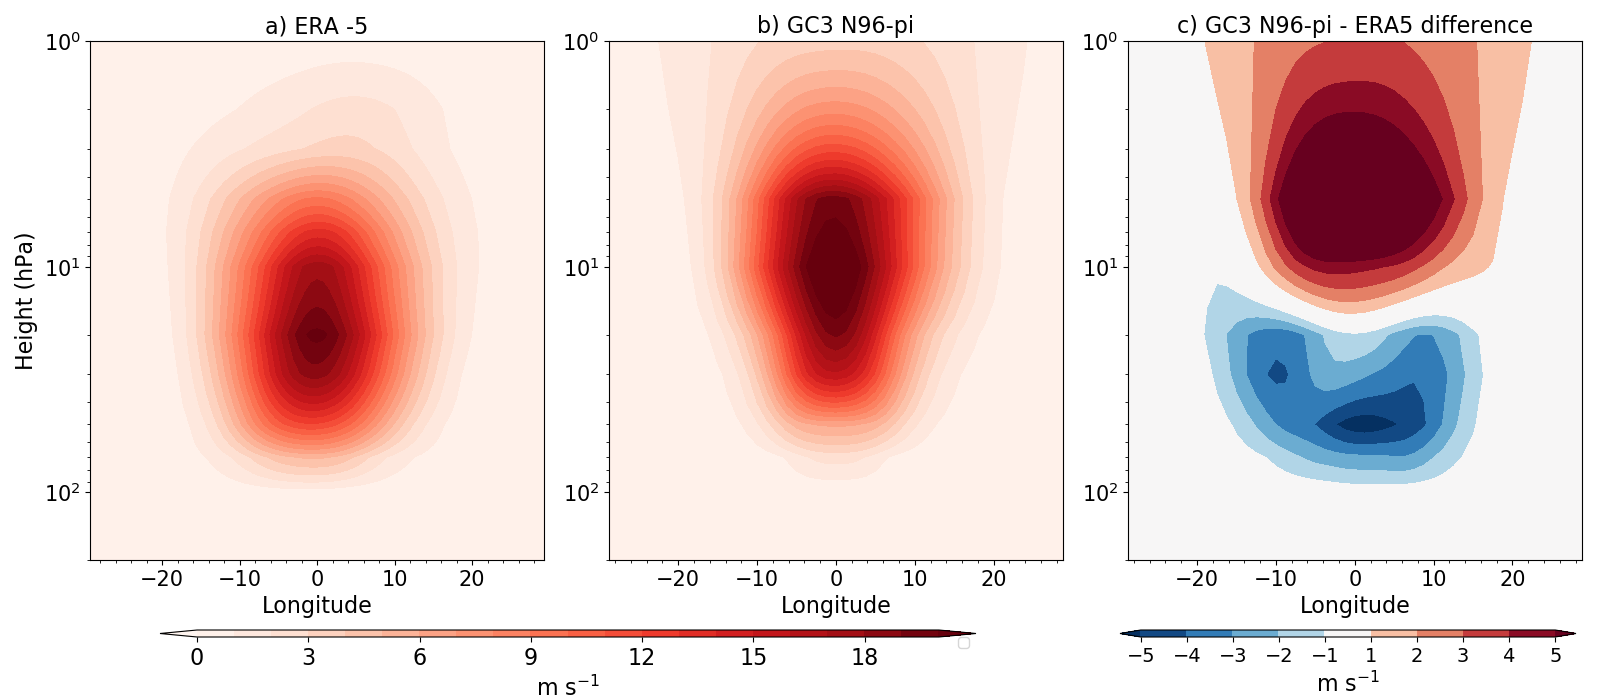
\includegraphics[width=\linewidth]{figures/qboamplitude.png}
\caption[QBO amplitude bias]{Latitude-pressure plot of the amplitude [m s$^{-1}$] of the QBO. Obtained from the zonal mean zonal wind fourier spectrum magnitude within the QBO periods, as in \cite{schenzinger2017}. }
\label{fig:qboamplitude}
\end{figure}

\subsection{The importance of biases in the UTLS for stratosphere-tropospheric coupling}

One key stratospheric bias in most of the existing climate models relates to the representation of the QBO in the lowermost stratosphere. Figure \ref{fig:qboamplitude} illustrates this bias in GC3 N96-pi by comparing the variation of the QBO amplitude  with height and latitude with ERA5; the amplitude is obtained using the method in \cite{schenzinger2017}. The amplitude of the QBO in the lowermost equatorial stratosphere is much smaller and extends to the subtropics less in the model than in ERA5, in agreement previous studies \citep{schenzinger2017,richter2020,bushell2020}. The implication of this bias is that if the QBO signal is too weak in the lower part of the stratosphere in the model, the simulated meridional circulation will also be weaker, and any temperature anomaly associated with this residual circulation will also be smaller near the tropopause. 

The main hypothesis suggested in the literature to explain observed relationships between the QBO and tropical convective diagnostics is the temperature variability in the tropopause layer and its influence on the upper-level static stability \citep[][]{collimore2003,liess2012,nie2015,gray2018}.
Models that simulate a weaker than observed variance of the temperature near the tropopause associated with the QBO may dampen any processes that relate the QBO to tropical convection.
Due to the fact that most models underestimate the variability of the temperature associated with the QBO in the UTLS region, several studies have argued in favour of performing numerical experiments with a GCM where the stratosphere is relaxed towards an observed or idealized state \citep[e.g.][]{lee2018,martin2021} to correct this bias. 

Chapter \ref{ch:7-qbo} described a number of robust signals in convective features associated with the QBO within the CMIP6 experiments that have an internally generated QBO. 
Figure \ref{fig:qboamplitude} shows that the signal that may be responsible for these relationships is too weak within these models. 
One might reasonably then expect that if the models simulate a stronger temperature variability associated with the QBO, then the surface response to the phase of the QBO would also increase. 
The remainder of this chapter describes the experimental design and results of simulations that aim to alleviate the biases in the QBO in the lower stratosphere and compare the surface response in these experiments with those of simulations with a free-running stratosphere with an internally generated QBO.
%The purpose of these experiments would be to improve the representation of stratospheric features such as the QBO in order to investigate how accurately representing these stratospheric oscillations can modify impacts elsewhere. 

The following section describes a nudging protocol using the Met Office Unified Model. The aim of these experiments is to investigate how the tropical route of QBO teleconnections is modified when the representation of the QBO is improved, and whether nudging is a good tool for this purpose.

\subsection{The nudging protocol}



This section describes the experimental setup for the nudging experiments. 
The GC3.1 configuration of the UM model is used (model version 11.4), using an atmospheric horizontal resolution of N96 (corresponding to the low-resolution version of the simulations of the MOHC submitted to CMIP6). 
Both atmosphere-only and ocean-atmosphere coupled experiments were conducted, in all cases spanning the period 1981-2015, using a present-day climate setup where all forcings are set constant to those of the year 2000, so there is no variation in, e.g., greenhouse gases within these simulations.

Nudging refers to the relaxation of a variable within the model to a specified state, and is a technique that has recently been used for several purposes such as investigating the MJO-QBO relationship in a climate model \citep{martin2021} and the role of the upper stratosphere for forecasting sudden stratospheric warming events \citep{gray2020}.

\begin{figure}[t!]
\centering
 %\noindent
 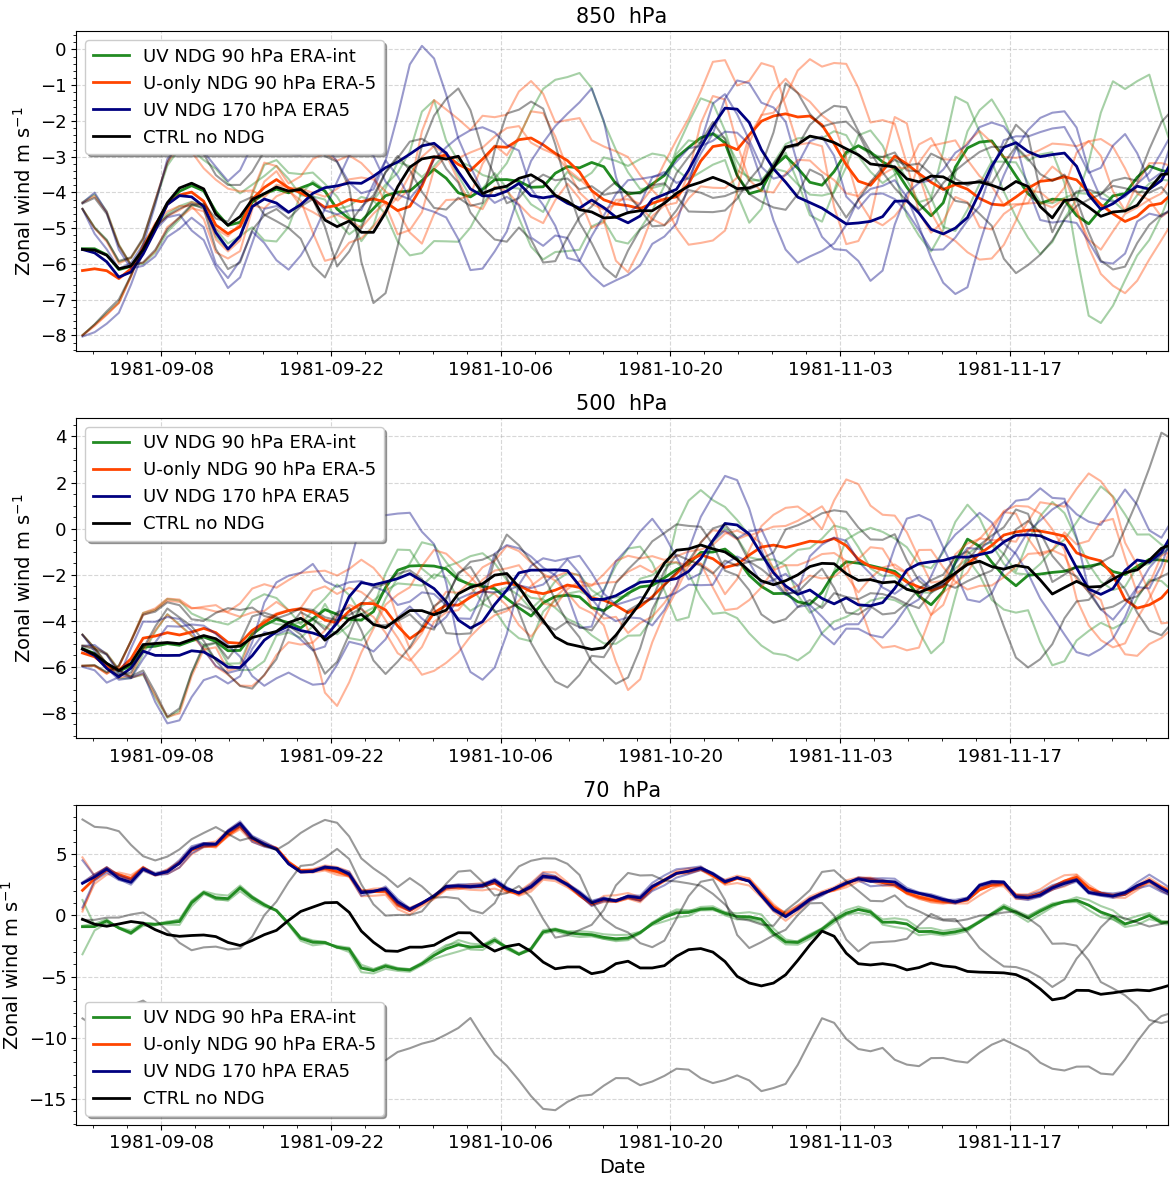
\includegraphics[width=0.95\linewidth]{figures/u_test__.png}
\caption[Time-series of zonal-mean winds under different nudging conditions]{Time-series of the zonal-mean zonal wind in the 10$^\circ$S-10$^\circ$N band at the 850 hPa (upper), 500 (middle) and 70 hPa (lower) levels. Results are from atmosphere-only simulations without nudging (CTRL no NDG), with nudging applied to both $u$ and $v$ up between 90 and 4 hPa using ERA-interim data (UV NDG 90 hPA ERA-int), with nudging between 170 hPa and 4 hPa nudging $u$ and $v$ using ERA5 data and finally, nudging only $u$ from 90 to 4 hPa using ERA5 data. For each kind of the simulation, each ensemble member is shown (faint line) and the ensemble mean (solid line) is shown. }
\label{fig:u_nudg_stv}
\end{figure}

In the UM setup, three variables can be relaxed, air temperature ($T$) and the zonal and meridional components of the wind ($u$ and $v$). The relaxation is applied towards reanalysis data or towars an idealized state at each grid-point, in contrast to the setup in other models \citep[e.g.][]{martin2021} where the relaxation is performed in a zonal-mean sense.
 Furthermore, the nudging can be performed between specified vertical levels and in selected latitude/longitude regions. % to certain levels within certain longitudes and latitudes using different reanalysis datasets or even idealized states. 
 To find the experimental setup that resulted in an improvement in the representation of the QBO without over constraining the model's climatological state we conducted several sensitivity tests using an atmosphere-only setup to test the effect of nudging all $u$, $v$ and $T$ compared to just one, as well as the model levels and latitudes where the nudging was applied. 


Figure \ref{fig:u_nudg_stv} shows the time-series of the zonal-mean zonal wind at different levels for the different sensitivity experiments performed. Three ensemble members were performed first for a control simulation with no nudging, a simulation where $u$ and $v$ were relaxed towards ERA-interim, and two simulations with ERA5 as the nudging data, one relaxing $u$ between 90-4 hPa and another relaxing $u$ and $v$ between 170 hPa and 4 hPa.


These results show that in the troposphere (850 hPa) all the ensemble members diverge towards different states, whereas in the lower stratosphere, the ensemble members of the nudged simulations converge towards a single state. The nudged simulations at the 70 hPa level differ only due to the nudging data, highlighting the differences in the zonal wind in the equatorial stratosphere between ERA5 and ERA-interim. 
From this part on, results using only ERA5 nudging data are presented. 

\begin{figure}[t!]
\centering
 %\noindent
 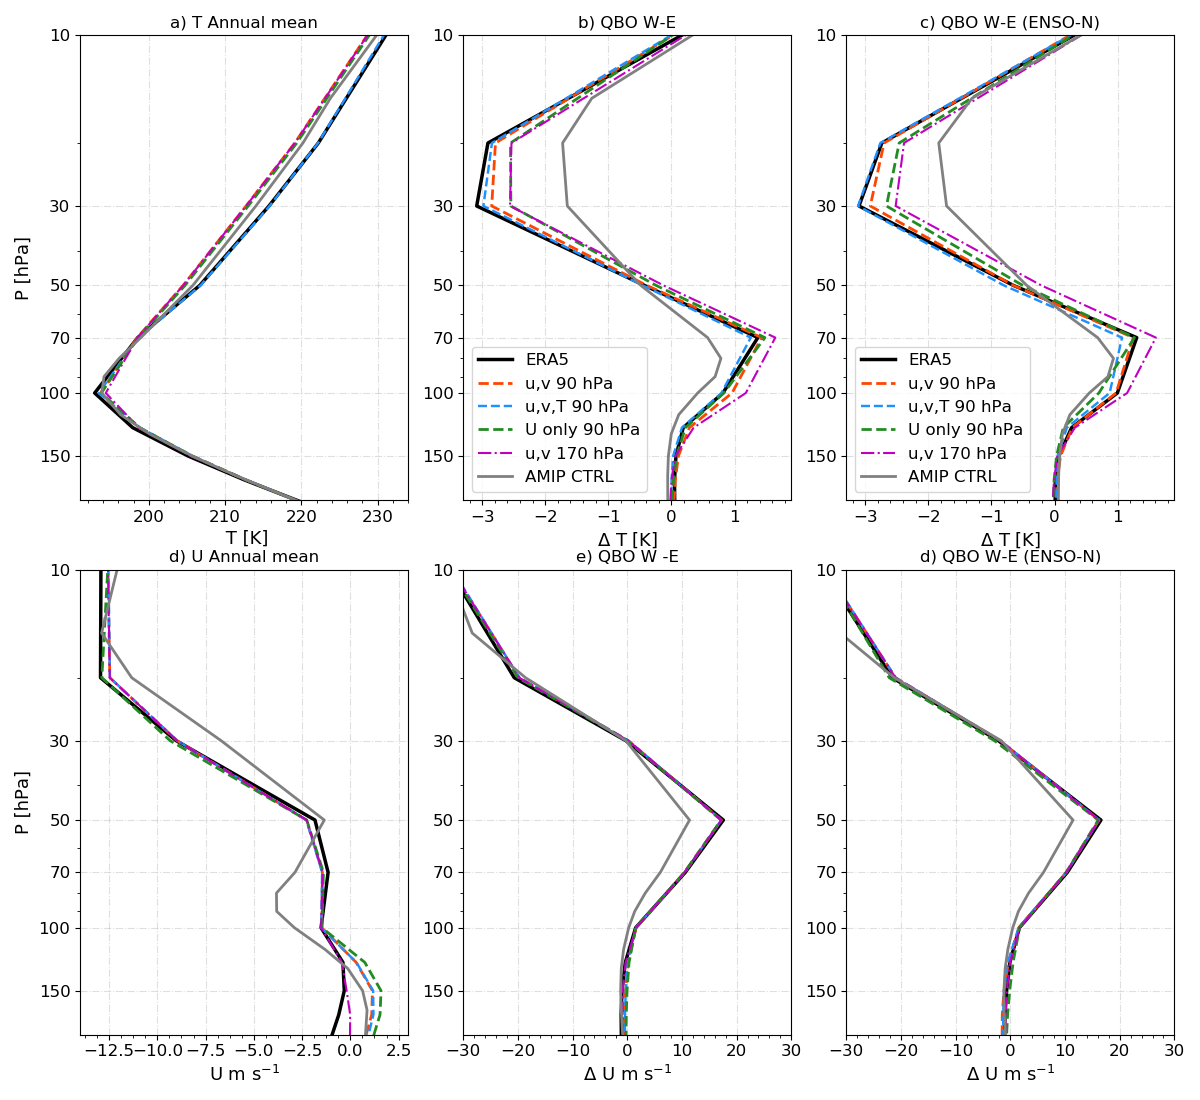
\includegraphics[width=\linewidth]{figures/profilUTclimatology.png}
\caption[Nudging sensitivity QBO profiles]{Vertical profiles of zonal mean temperature (a-c) and zonal wind (d-f) depicting the climatological state (a, d), the QBO W-E difference (b, e) and the QBO W-E difference during Neutral states of ENSO (c, f). In all the simulations with relaxation, the nudging data was ERA5.}
\label{fig:prof_nudg}
\end{figure}

Figure \ref{fig:prof_nudg} shows the vertical profiles of temperature and zonal wind in these simulations. The variability of $T$ associated with the QBO, is fairly well represented by all the nudged simulations, compared to the control simulations, even when $T$ was not relaxed towards ERA5. This results proves that the meridional circulation imposed by the shear imposed when relaxing $u$ is enough to force temperature variability within the model through thermal wind balance, as found in \cite{martin2021}. 

The climatological zonal mean zonal wind and the variability of associated with the QBO (Fig. \ref{fig:prof_nudg}d-f) is much improved in the simulations with nudging, as expected, in the stratosphere. Notably, in the simulations where nudging was applied above 90 hPa, the biases lower down in the stratosphere at 150 hPa remain comparable to those of the control simulation, indicating that nudging the stratosphere does not pose a direct effect over the upper-tropospheric climatological state, in a zonal-mean sense.

 % and different variables were relaxed. 

The final experimental design chosen was to perform the nudging in the model levels 52-72 which roughly correspond to 90 hPa to 4 hPa, with a tapering of 4 levels, which means that full nudging was only working within levels 56-68. The nudging was done at all longitudes in the latitude band of 10$^\circ$S-10$^\circ$N with a latitudinal tapering of 10 degrees on both sides. Only the zonal component of the wind ($u$) was relaxed, so that $T$ and $v$ were not relaxed. 
The experimental setup aims to reasonably simulate the observed variability of the zonal wind leaving the meridional component of the wind and the temperature to respond freely within the model. 

Atmosphere-only and coupled ocean-atmosphere simulations were performed with this nudging setup, with corresponding control simulations in which there was no relaxation of any kind. The atmosphere-only, also referred to as AMIP, experiments were run with observed SSTs from the HadSST dataset. In all cases the nudging of the atmosphere was done only between 90 and 4 hPa and at equatorial latitudes only, whereas the surface boundary SSTs are used at all latitudes.
For the nudged experiments several ensemble members were performed, three for the atmosphere-only configuration and six for the coupled ocean-atmosphere configuration. Each ensemble member was initialized from a different ocean/atmosphere initial condition in order to decrease the role that internal variability may have on these simulations. 

\begin{table}[t!]
\caption{Experimental setup indicating the model configuration, the period, ensemble members, acronym and relaxation details.}
\begin{tabular}{p{2.3cm}|p{2.3cm}|p{1.73cm}|p{3cm}|p{5cm}}
Setup           & Period    & Ensemble members & Name            & Nudging                                          \\ \hline \hline
Atmosphere-only & 1981-2015 & 3                & AMIP            & ERA5. U-only 90 hPa                              \\
Atmosphere-only & 1981-2015 & 1                & AMIP-Control    & No                                               \\
Atmosphere-only & 1981-2015 & 3                & AMIP-Shifted    & ERA5. U-only, 90 hPa. Relaxation shifted -1 year. \\
Coupled         & 1981-2015 & 6                & Coupled         & ERA5. U-only 90 hPa.                             \\
Coupled         & 1981-2015 & 2                & Coupled Control & No.                                             
\end{tabular}
\end{table}

In addition to the nudged and control coupled and AMIP experiments, we performed another atmosphere-only experiment. In the normal AMIP Nudged experiment, the SST driving data corresponds to the zonal wind in the equatorial stratosphere that was observed in the real-world. To explore possible feedback processes between QBO winds and the SSTs, we performed an AMIP Shifted experiment, where the nudging data was shifted with a -1 year lag from the SSTs. In this experiment, e.g., the model year 1997 was run using 1997 SSTs but zonal winds in the stratosphere corresponding to 1996 of ERA5. In this way we have minimised any in-phase relationship between the QBO phase and the SSTs. An alternative approach would be to 'shuffle' the SSTs so that each year is run with randomly selected SSTs. However, since we are performing multi-year simulations this has associated issues of how to join the randomly-selected SSTs at the year-boundary, to form a coherent multi-year SST time-series. To avoid this issue we decided to simply shift the SSTs by one year so the QBO phase and SSTs were not aligned.  

The following section presents the results of these experiments, first by reporting how the tropical tropopause variability is modified when nudging is applied and then by showing the surface impacts associated with the QBO in the nudged experiments, first in the atmosphere-only configuration and then in the coupled setup.

\begin{figure}[t!]
\centering
 %\noindent
 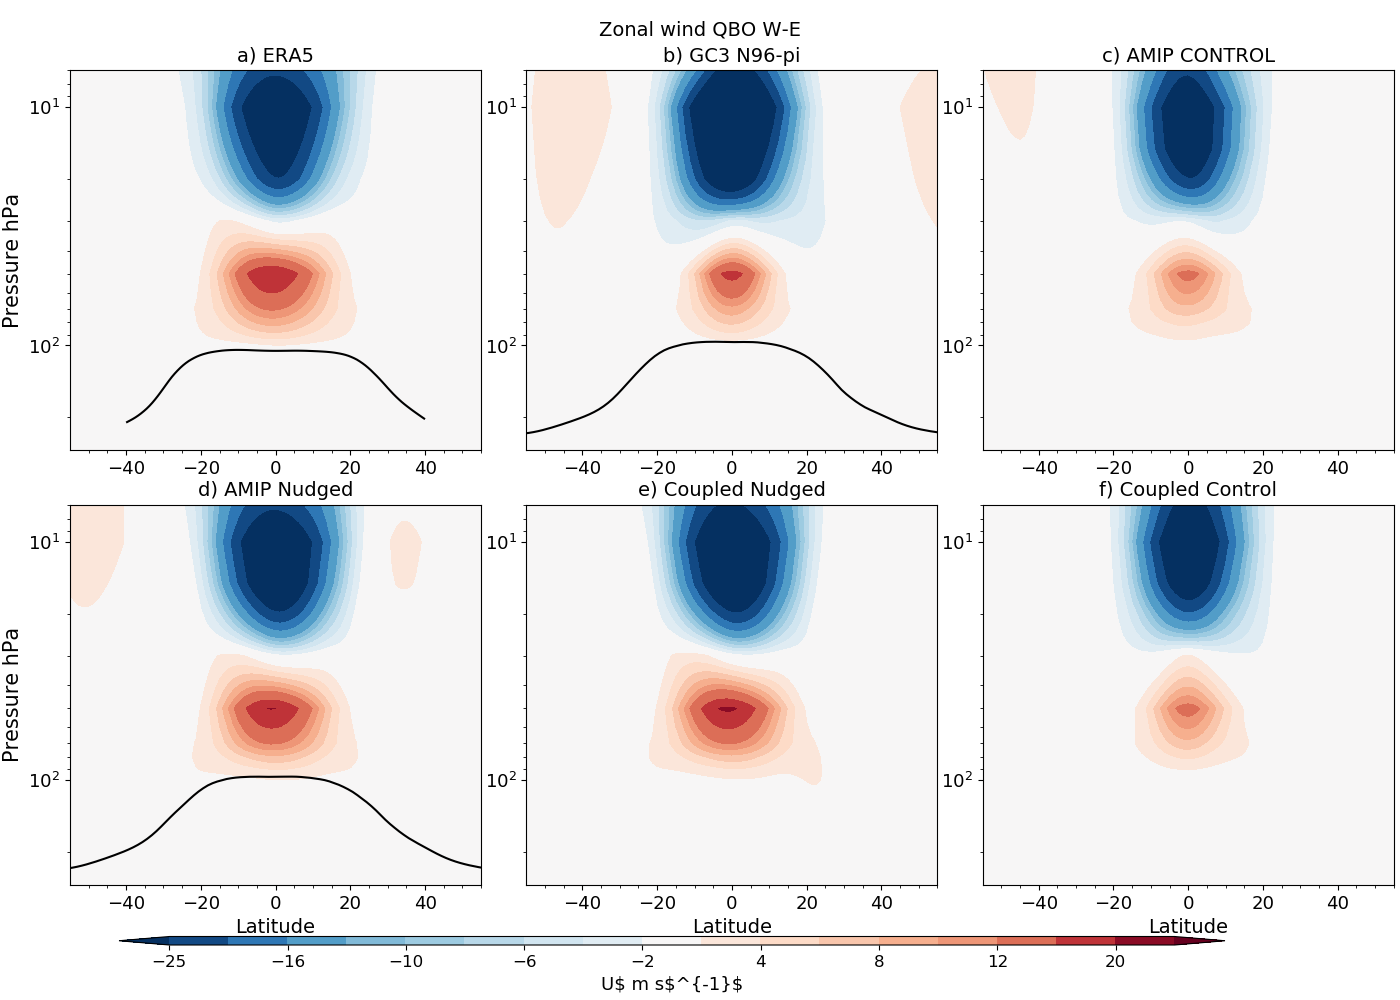
\includegraphics[width=\linewidth]{figures/zonalplotx_wind.png}
\caption[Zonal mean zonal wind QBO difference]{Latitude-height plot of the zonal-mean zonal wind differences (QBO W-E) in (a) ERA5, (b) GC3 N96-pi from CMIP6, the control simulations with no nuding in an (c) AMIP and (f) coupled configurations, and the nudged simulations in (d) AMIP and (e) coupled configurations. The black line denotes the tropopause height obtained from the model data in (b, d) and for ERA5 the tropopause height was found through the gradient threshold method. For the nudged experiments, the ensemble-mean is shown. }
\label{fig:zonal_u}
\end{figure}

\section{ Results from nudging experiments}




This section investigates the effect of nudging for the representation of the QBO, the variability in the upper troposphere lower stratosphere (UTLS) associated with the QBO, and ultimately, surface impacts driven by QBO effects on tropical convection. 
First, this section evaluates how nudging modifies the wind and temperature variability in the UTLS region compared to control and CMIP6 simulations.  



\subsection{Tropical UTLS variability}


Figure \ref{fig:zonal_u} shows the zonal mean difference in zonal wind associated with the QBO phase, in a latitude-height sense, in the 500-y CMIP6 GC3 N96-pi and both the AMIP and coupled 35-year (un-nudged) control simulations. The zonal wind variability in the lower stratosphere associated with the QBO is deficient in the GC3 N96-pi and control experiments, principally near the tropopause as the signal is too narrow and weaker than in the reanalysis.
 
\begin{figure}[t!]
\centering
 %\noindent
 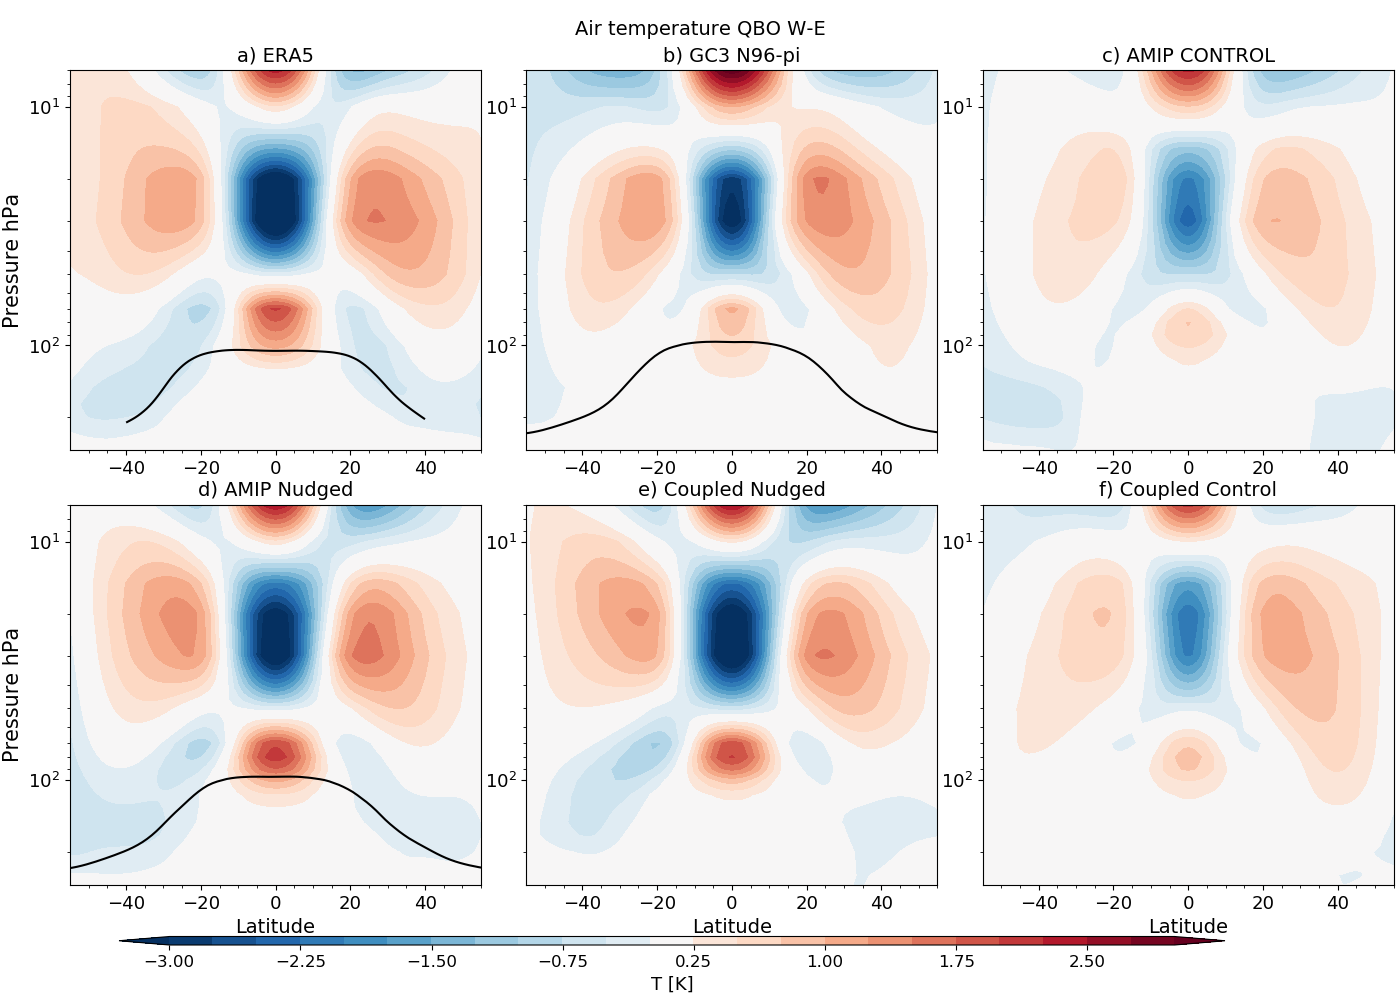
\includegraphics[width=\linewidth]{figures/zonalplotair_temperature.png}
\caption[Zonal mean air temperature QBO difference]{As in Figure \ref{fig:zonal_u} but for air temperature.  }
\label{fig:zonal_T}
\end{figure} 

 %The variability in the mid-stratosphere winds is also improved as the signal is wider reaching the subtropics. This means that the representation of shear, which modulates temperature as well, is improved with the nudging in the 20$^\circ$S-20$^\circ$N.



The temperature is able to respond to the nudging within the model freely, Figure \ref{fig:zonal_T} reveals that nudging the zonal wind can also improve the air temperature variability in the lower stratosphere driven by the QBO shear. The positive temperature anomaly in the equatorial region around the 100 hPa at the tropopause level is much weaker in the GC3 N96-pi, AMIP Control and Coupled Control compared to the two nudged experiments and to ERA5. The Nudged experiments not only improve the temperature signal in the equatorial lower stratosphere but seem to overestimate this signal around the 70 hPa level. 

However, observations show a horse-shoe temperature anomaly pattern in the subtropics characterised by a negative anomaly that extends from 20-40 degrees north and south, a signal that is missing in the GC3 N96-pi, AMIP Control and Coupled Control experiments but is recovered in the Nudged experiments. This means that without nudging further away than 20 degrees north or south, the subtropical signal is obtained by improving the residual circulation associated with the QBO. 

\begin{figure}[t!]
\centering
 %\noindent
 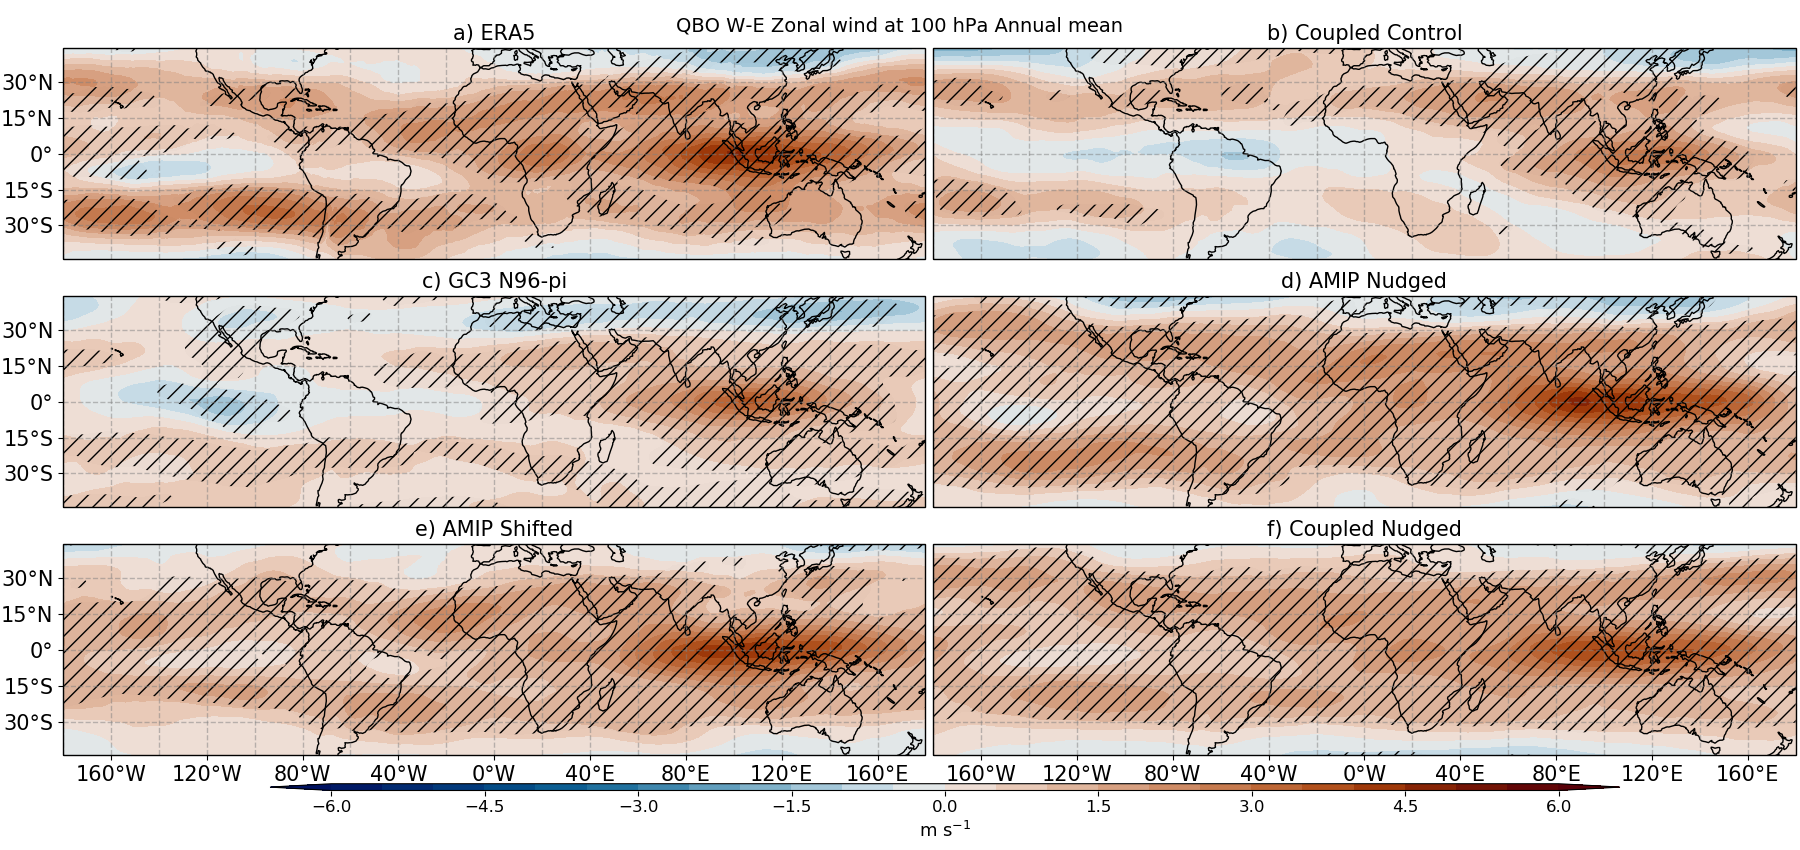
\includegraphics[width=\linewidth]{figures/ua100climqbowf.png}
\caption[Zonal wind QBO W-E difference 100 hPa level]{Zonal wind difference in QBO W-E at the 100 hPa level. Hatching denotes significance to the 95\% level according to a Student's t-test.}
\label{fig:ua100qbo}
\end{figure}

The spatial distribution of the wind and temperature variability associated with the QBO near the tropopause level (100-hPa level) is shown in Figures \ref{fig:ua100qbo} and \ref{fig:ta100qbo} for ERA5, GC3 N96-pi and control and nudged experiments. 
These Figures show, first, that the free running model (seen in GC3 N96-pi and Coupled Control) is able to reproduce the zonal asymmetries in the QBO signal \citep{tegtmeier2020b} at the 100 hPa level albeit much weaker than the observed signal. The wind differences, for instance, are stronger over the Maritime continent in observations whereas the temperature signal is stronger in the Maritime continent and over equatorial Africa, both features reproduced sensibly by the model without nudging. 

The nudging particularly improves the temperature response to the QBO at 100 hPa where the QBO W-E difference is more than twice the amplitude of the un-nudged response. 
%increases the magnitude of these signals at the 100 hPa level, both for the zonal wind and the temperature differences. 
In addition, the temperature signal in the Nudged experiments is improved in AMIP Nudged and AMIP Shifted experiments, indicating that these differences are not associated with the underlying SST field, rather with the QBO vertical wind shear, which has been improved by nudging. 
Results found in this analysis also indicate that the tropopause height and temperature exhibits more variability associated with the QBO than in the free-running model (not shown). 


\begin{figure}[t!]
\centering
 %\noindent
 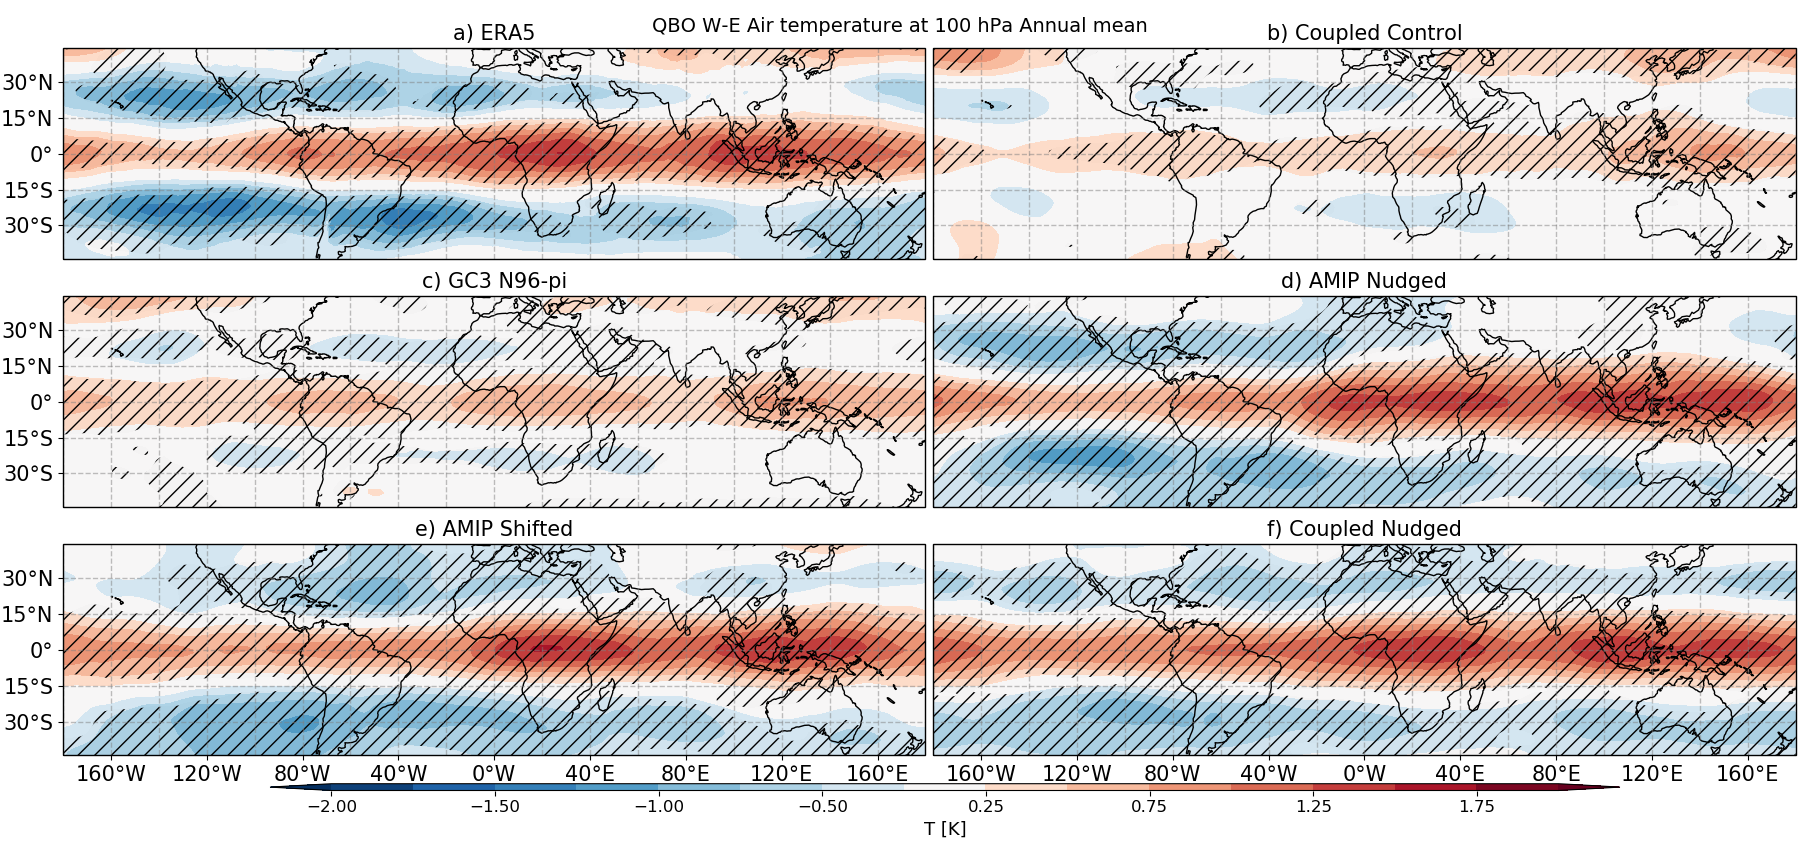
\includegraphics[width=\linewidth]{figures/ta100climqbowf.png}
\caption[Zonal wind QBO W-E difference 100 hPa level]{As in Figure \ref{fig:ua100qbo}, but for air temperature. }
\label{fig:ta100qbo}
\end{figure}

This section shows that the UTLS temperature and zonal wind variability are more realistic in the nudged experiments, and that this variability is not related to the underlying SSTs but rather a result of the relaxation in the equatorial stratosphere. These results indicate that these experiments are suited to investigate tropical teleconnections associated with the QBO. The hypothesis to test is that the processes that link the QBO to tropical convection should be more realistically represented in the nudged experiments than in the control experiments. %The following section investigates whether in fact surface impacts in the tropics are stronger in the nudged experiments compared to free-running simulations. 

\begin{figure}[b!]
\centering
 %\noindent
 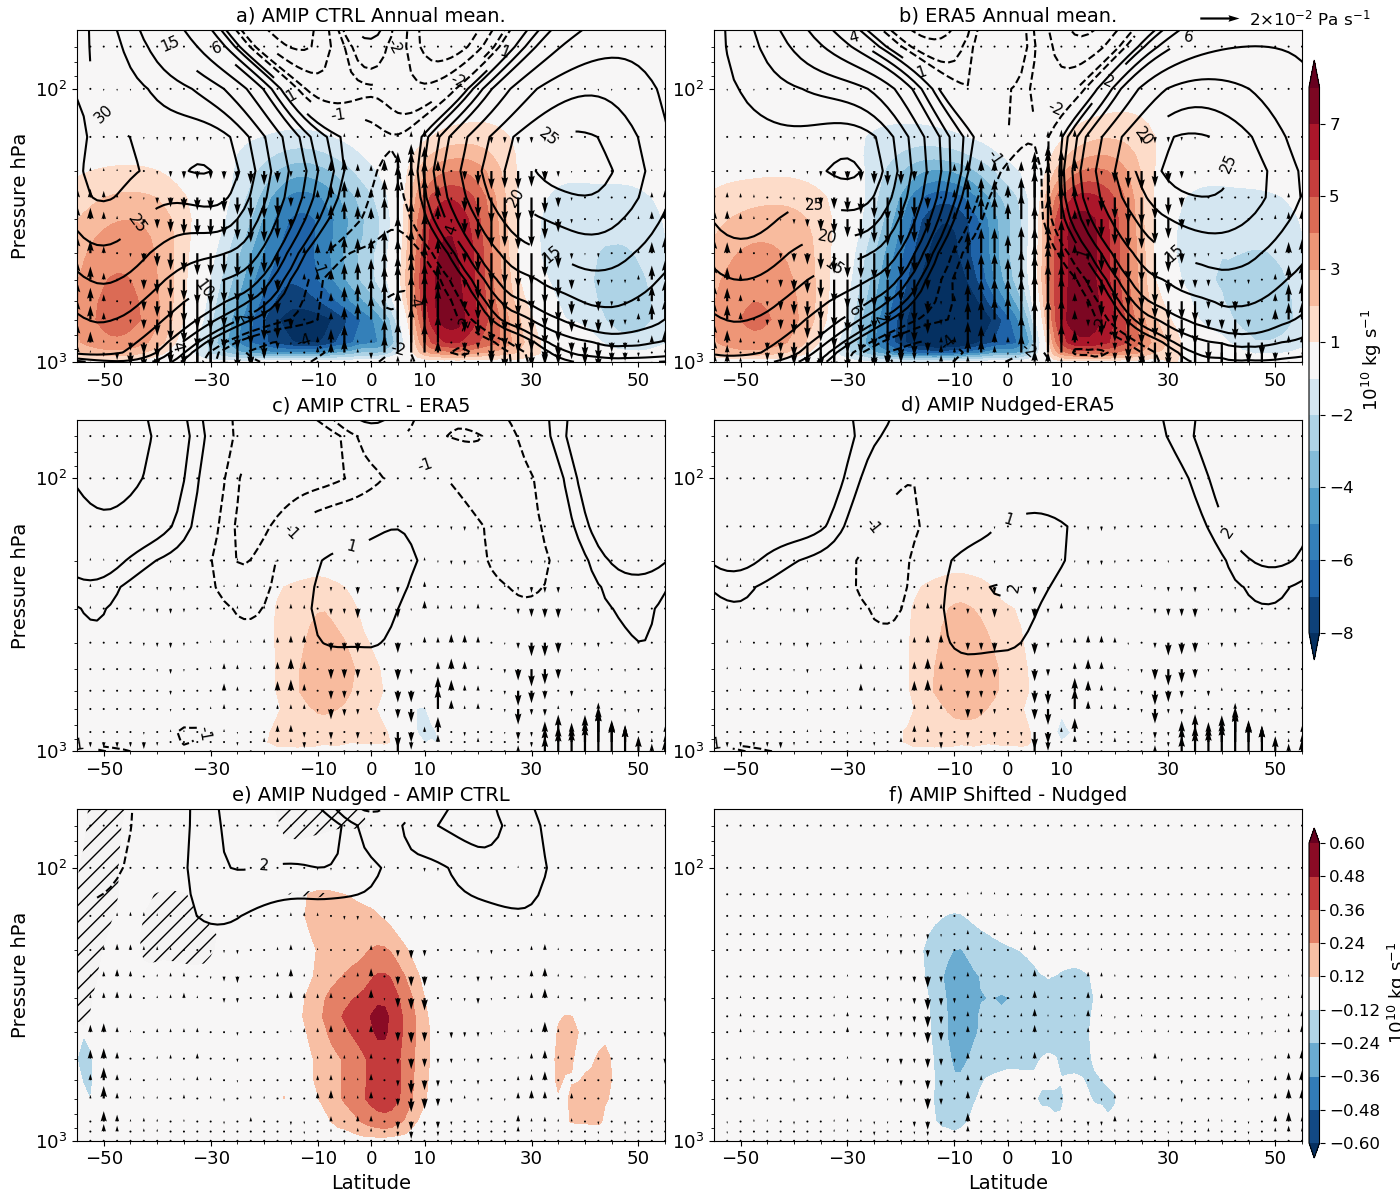
\includegraphics[width=\linewidth]{figures/suite_streamhadleyclim.png}
\caption[Hadley cell in atmosphere-only experiments]{Hadley cell meridional mass streamfunction (shading), zonal mean zonal wind (contours in m s$^{-1}$) and vertical velocity (vectors). Climatological mean in the (a) AMIP Control experiment and (b) ERA5. (c-d) show biases in the (c) Control and (d) Nudged experiments with respect to ERA5 whereas (e-f) show differences between experiments, (e) AMIP Nudged-Control and (d) AMIP Shifted-Nudged. Note that the colorbar and scale of the vectors changes are different between (a-d) and (e-f). In (e-f), significant differences (95\% confidence level according to a Mann-Whitney two-sided test) in the streamfunction are highlighted with hatching . }
\label{fig:hadleyamip}
\end{figure}

\subsection{Atmosphere-only experiments}



This section describes the results of the atmosphere-only experiments: AMIP Nudged, AMIP Control and AMIP Shifted. These simulations use the CMIP6 SST dataset used for AMIP experiments, i.e.,  the SSTs in these runs follow the observed seasonal and interannual variability of SSTs. 
The effect of nudging on the tropical circulation and precipitation is shown in the following sections. % is first described to evaluate whether nudging has significantly modified the mean state of the Hadley and Walker circulations. Then, the precipitation response to the QBO is compared between Nudged and Control AMIP simulations.

\subsubsection{The tropical circulation}

\begin{figure}[b!]
\centering
 %\noindent
 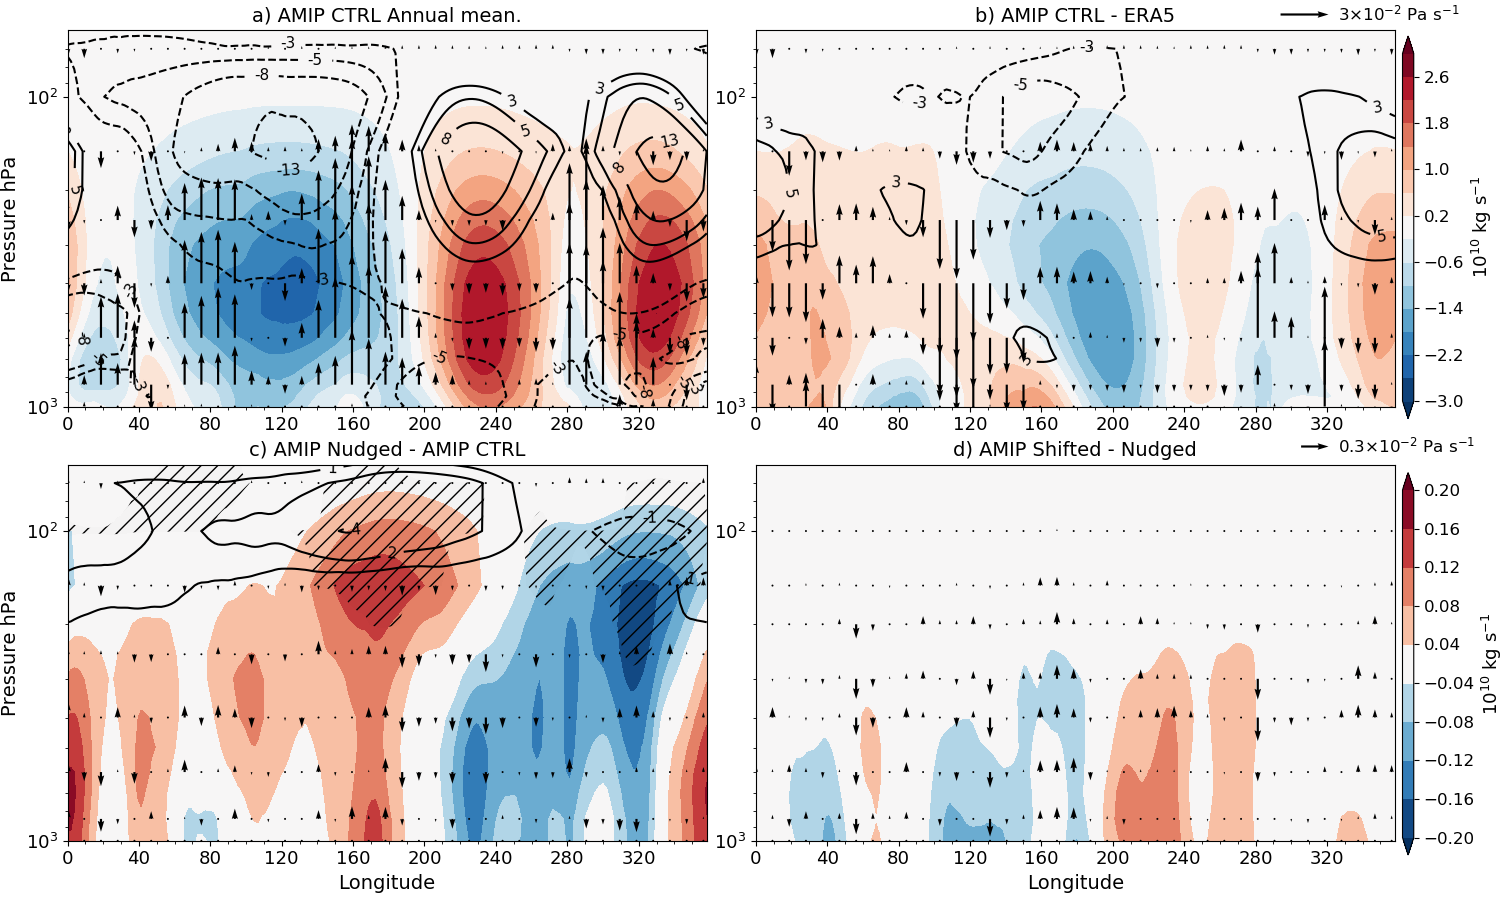
\includegraphics[width=\linewidth]{figures/suite_streamwalkerclim.png}
\caption[Walker in atmosphere-only experiments]{Zonal mass streamfunction ($\psi$ in shading), zonal mean zonal wind (contours) and vertical velocity (vectors) averaged over the 10$^\circ$S-10$^\circ$N, as in Figure \ref{fig:hadleyamip}. }
\label{fig:walkeramip}
\end{figure}

The mean state of the Hadley cell in the atmosphere-only configuration is weaker than in ERA5 in the 20$^\circ$S-0$^\circ$ region and there are also biases in the equatorial upper-level tropical and subtropical troposphere where the model shows an easterly bias (Fig. \ref{fig:hadleyamip}). 
The AMIP Nudged simulation shows  positive zonal wind differences with the Control experiment in the UTLS region, i.e, improving the easterly biases of the Control experiment. However, no significant differences in the streamfunction over the tropical troposphere are observed. Similarly, no significant differences were found in the mean-state of the Hadley circulation between the Nudged and Shifted experiments (Fig. \ref{fig:hadleyamip}f), suggesting that the variability of the nudging data is of secondary importance relative to the SSTs and the mean state of the nudging data. 

In turn, the Walker circulation biases in the upper troposphere are notably improved in the Nudged experiment (Figure \ref{fig:walkeramip}). The mean state of the Walker circulation is weaker in the AMIP Control simulation compared to ERA5, characterised by a weaker circulation in the Western Pacific and an easterly bias at upper levels. These two tropospheric biases in the Control experiment are reduced in the Nudged experiments, the relaxation is only applied above 90 hPa although significant differences in the zonal wind and zonal streamfunction are observed at 200 hP near the dateline, over South America and over the Atlantic Ocean. 
However, no significant differences in the streamfunction or zonal wind in the lower troposphere are observed between the AMIP Shifted and Nudged experiments which means that the mean overturning circulation is not modified by the variability of the nudging data.

\begin{figure}[b!]
\centering
 %\noindent
 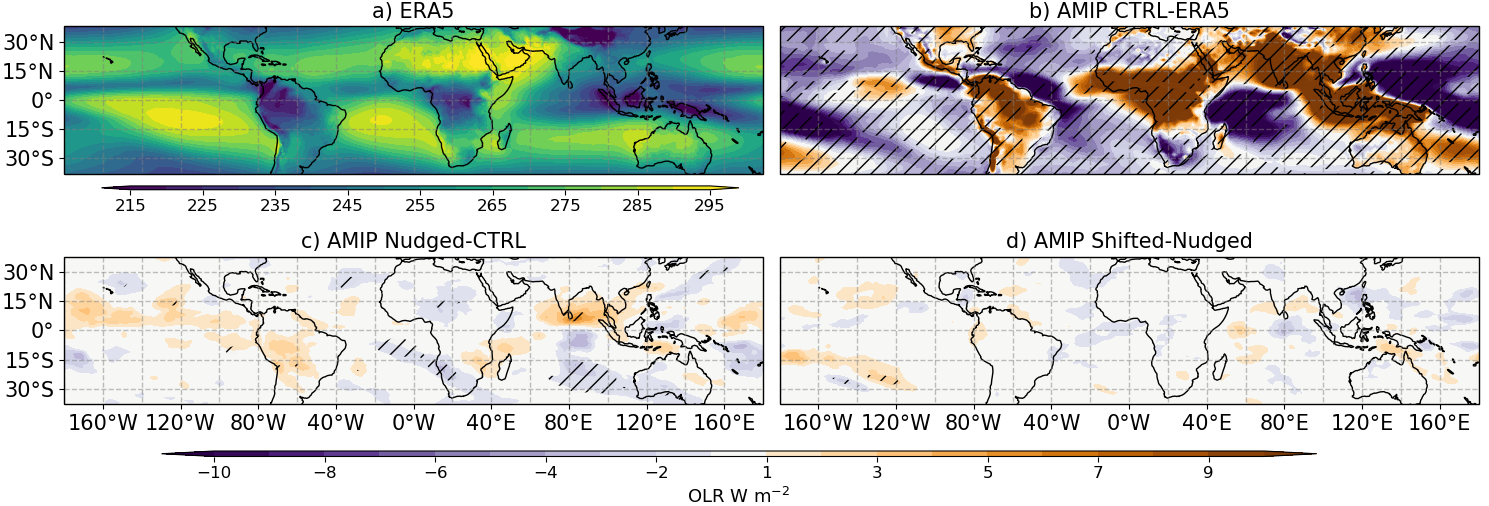
\includegraphics[width=\linewidth]{figures/olr_check.png}
\caption[Annual mean OLR  in atmosphere-only experiments]{(a) Climatological mean OLR [W m$^{-2}$] in ERA5, (b) climatological biases in the AMIP Control simulation. (c) Differences between AMIP Nudged and Control and (d) between AMIP Shifted and Nudged. Significant (95\% confidence level) differences according to a Mann-Whitney U test in (c, d) are highlighted with hatching. }
\label{fig:olr-mean}
\end{figure}

In spite of the fact that nudging reduces biases in the mean state of the Hadley and Walker circulation at upper levels, these reductions are small relative to the magnitude of the biases. 
Therefore, it remains unclear whether the nudging has significantly modified other aspects of tropical climate. 
An examination of the climatological  OLR in the tropics (Figure \ref{fig:olr-mean}) shows that most regions in the tropics exhibit significant and relatively large biases in AMIP Control compared to ERA5, most of which remain unchanged in the AMIP Nudged and Shifted experiments. The small and not significant differences between the Shifted and Nudged experiments suggest a small effect of the relaxation of the zonal winds over the mean state of OLR. 

\begin{figure}[b!]
\centering
 %\noindent
 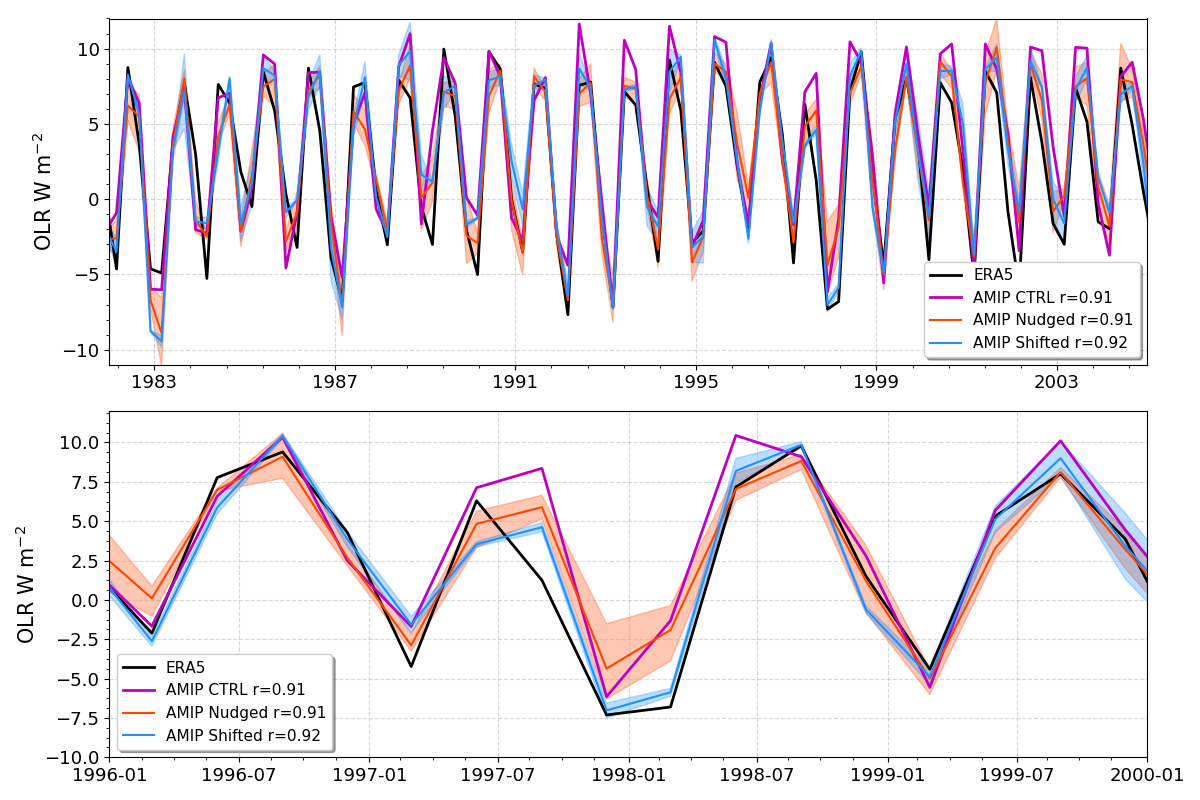
\includegraphics[width=\linewidth]{figures/olr_tseries.png}
\caption[Tropical mean OLR time series.]{Time-series of zonal-mean equatorial [5$^\circ$S-5$^\circ$N]  OLR in ERA5 and the three amip experiments for (a) 20 yrs and a (b) 5-yr period around the 1997-1998 ENSO event. For each AMIP experiment the Pearson correlation coefficient between the experiment time-series and ERA5 is shown in the legend. }
\label{fig:olramip_tseries}
\end{figure}



Similarly, Figure \ref{fig:olramip_tseries} shows that the zonal-mean OLR time-series averaged over the deep tropics is indistinguishable between the three AMIP experiments, and the time-series of all the experiments have the same correlation coefficient with ERA5. In other words, the tropical mean OLR remains unchanged in the nudged experiments, regardles of whether the relaxation was implemented to match the SST field or whether the nudging data was shifted from the SST time-series. 
Based on these results alone, it would appear that nudging has made little impact over the interannual variability of the tropical mean OLR. 
%The question of whether the specific variability of OLR and precipitation associated with the QBO is also the same is now investigated in the next section. 


\subsubsection{Precipitation response to the QBO}

\begin{figure}[t!]
\centering
 %\noindent
 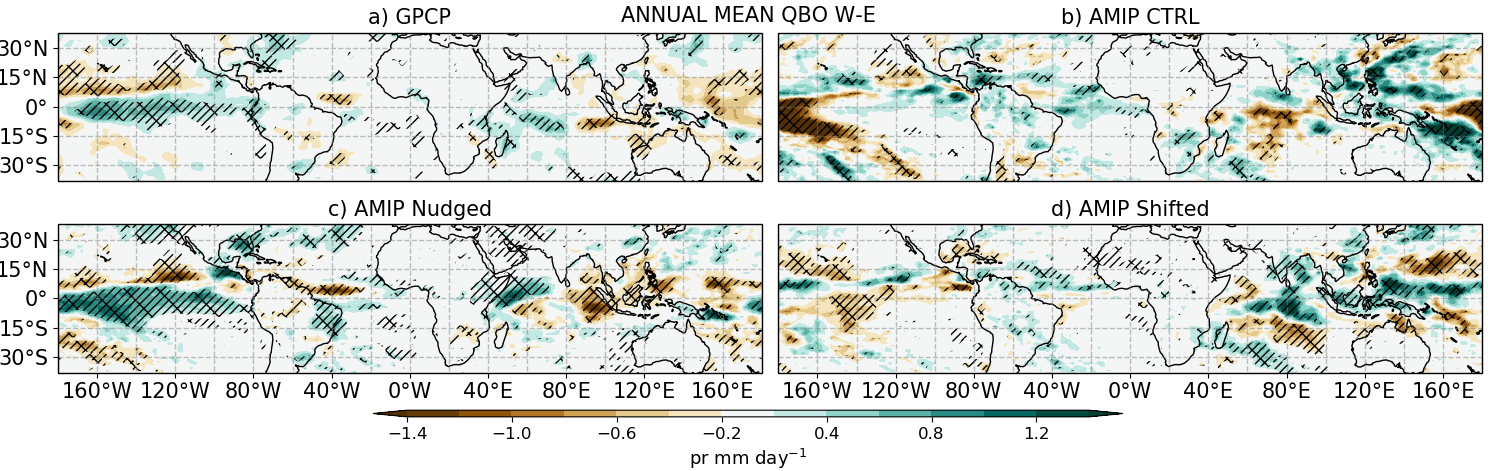
\includegraphics[width=\linewidth]{figures/pr_amip_climqbowqboe.png}
\caption[Annual mean precipitation response in atmosphere-only experiments]{Annual-mean precipitation response (QBO W-E) in (a) GPCP, and atmosphere-only experiments: (b) AMIP CTRL, (c) AMIP Nudged and (d) AMIP Shifted.  }
\label{fig:amip_clim}
\end{figure}


The annual-mean difference of precipitation between QBOW and E phases (Fig. \ref{fig:amip_clim}) in the ensemble-mean AMIP Nudged experiment matches closely the results of GPCP, characterised by an El Niño pattern in the Pacific Ocean, a weaker Atlantic ITCZ and a gradient of precipitation in the Indian Ocean during QBOW compared to QBOE. 
In contrast, the free-running AMIP Control and the simulations with an out-of-phase relaxation of the winds with respect to the SST driving data (AMIP Shifted) show very different responses to the AMIP Nudged experiment and observations. 

\begin{figure}[t!]
\centering
 %\noindent
 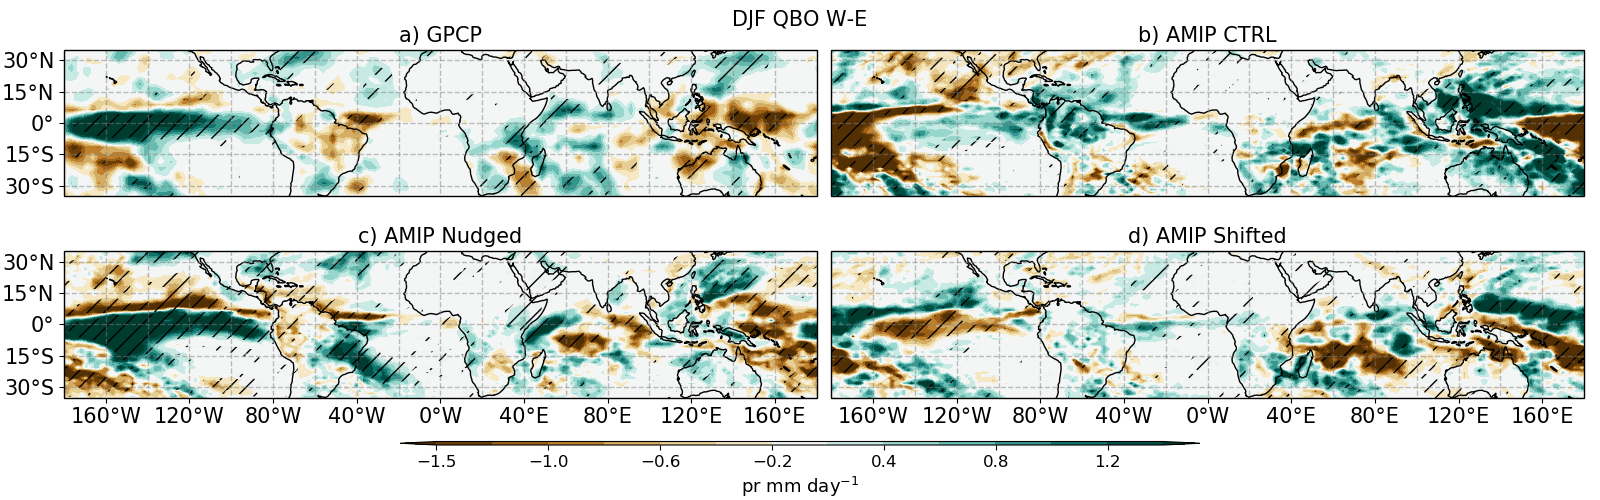
\includegraphics[width=\linewidth]{figures/pr_amip_djfqbowqboe.png}
\caption[DJF mean precipitation response in atmosphere-only experiments]{As in Fig. \ref{fig:amip_clim} but for the DJF season. }
\label{fig:amip_djf}
\end{figure}

A similar result is found when the composite differences only include DJF (Fig. \ref{fig:amip_djf}), so that the precipitation response in the simulations where the QBO index and the SSTs match exactly as in observations (AMIP Nudged) produce a very similar response to GPCP, whereas simulations where the QBO winds do not match the same SSTs result in different responses. 
Results using OLR are very similar, for example, Figure \ref{fig:amip_son_olr} shows that a strong response is diagnosed in GPCP in the Indian Ocean which is reasonably reproduced in AMIP Nudged but AMIP CTRL and AMIP Shifted exhibit a very different response in the Indian Ocean and elswhere.



These results suggest that the QBO winds are secondary to the effect of the SSTs for the precipitation response in these atmosphere-only experiments. The AMIP Shifted experiment has a better representation of the stratospheric variability in temperature and vertical wind shear, however, the response is entirely different to the AMIP Nudged experiments, the difference between these two experiments being the underlying SSTs. These results suggest that improving the representation of the QBO is not enough to replicate the observed response because the SST forcing dominates. 

\begin{figure}[t!]
\centering
 %\noindent
 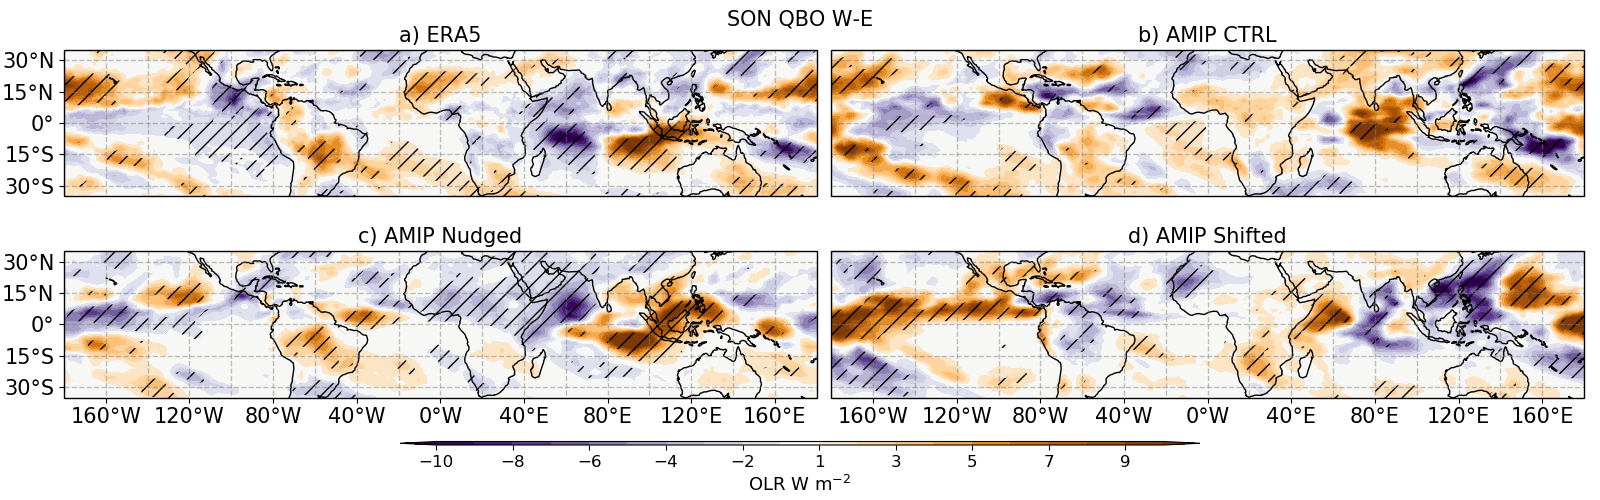
\includegraphics[width=\linewidth]{figures/olr_amip_sonqbowqboe.png}
\caption[SON OLR response in atmosphere-only experiments]{As in Fig. \ref{fig:amip_clim} but for OLR in the SON season. }
\label{fig:amip_son_olr}
\end{figure}

This section shows, first, that relaxing the zonal wind in the stratosphere in atmosphere-only experiments does not modify the mean state of the tropical circulation. Second, that the surface response of precipitation associated with the QBO in observations is largely associated with the underlying SSTs. The tropical mean OLR and precipitation mean state appear to be undistinguishable between Control, Nudged and Shifted experiments, whereas the composite differences between the two phases of the QBO reveal that the observed precipitation response is associated mostly with the SST anomaly pattern. However, whether the QBO has any effect over the SSTs cannot be answered in this atmosphere-only experiments, which leads to the the next section which analyses the coupled nudged experiments. 

\subsection{Coupled experiments}




This section presents the results of the coupled ocean-atmosphere experiments with (Nudged) and without (Control) relaxing the zonal wind in the tropical stratosphere. Note that all the individual experiments in this section are the same length (35 yr) and that the Coupled Nudged  ensemble-mean refers to the mean results of the six ensemble members with nudging and the Control ensemble-mean to the mean of the two ensemble members.
These coupled experiments differ only slightly from the setup used in the CMIP6 piControl experiments, analysed in section \ref{sq:cmip6_qbo}, with the atmospheric resolution of the nudged experiments matching the resolution of GC3 N96-pi (1.875$^\circ$x1.25$^\circ$) and the oceanic resolution of these resolutions being the same as GC3 N216-pi (0.25$^\circ$). The forcing is constant in both types of runs, except that in the piControl experiments, the forcing represents conditions of the year 1850 and in the nudged experiments of the year 2000. 
Due to these similarities, we compare the long-term CMIP6 experiments with the nudging experiments in some instances.

\begin{figure}[t!]
\centering
 %\noindent
 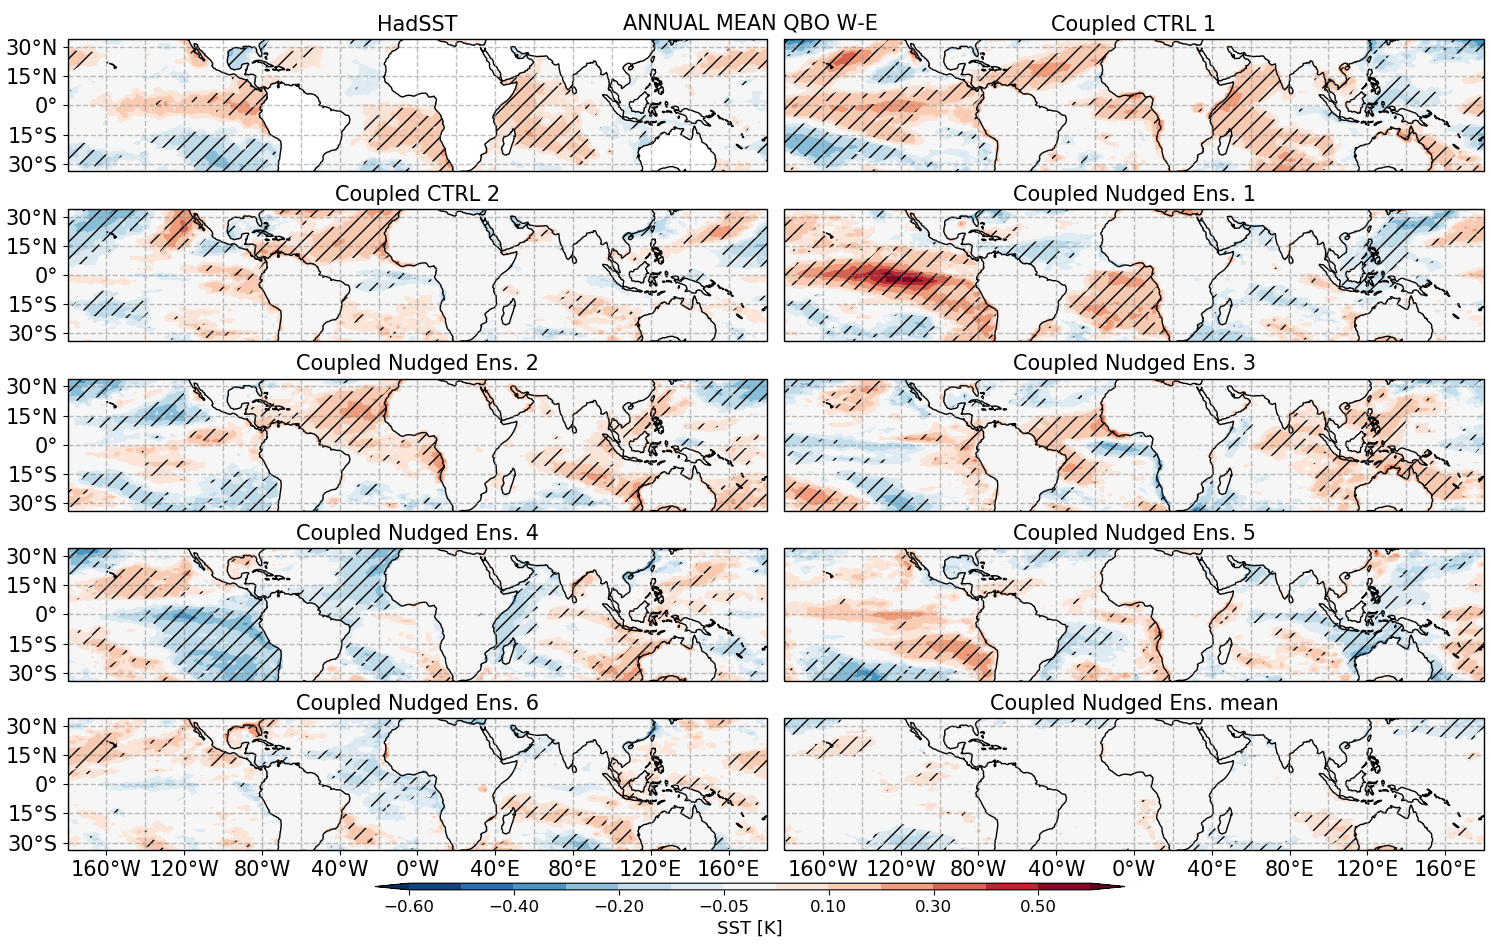
\includegraphics[width=\linewidth]{figures/sst_check_climqbowqboe.png}
\caption[Annual mean SST response to the QBO in coupled nudged experiments]{ Annual mean SST [K] QBO W-E differences in the HadSST dataset and the Coupled Control, Coupled Nudged ensemble members and the Coupled Nudged ensemble mean. Hatching denotes significance to the 95\% confidence level according to a bootstrapping with replacement test.}
\label{fig:sst_clim_coupled}
\end{figure}

\subsubsection{SST response}



The previous section shows that in atmosphere-only experiments the SST forcing dominates over any effect of the nudging, indicating that the mechanism by which the QBO influences tropical climate involves the SSTs. In the coupled ocean-atmosphere experiments, the SSTs are able to respond and interact with any atmospheric forcing, and for that reason, this section first presents the annual mean and seasonal mean differences between the two phases of the QBO comparing coupled nudged and control experiments. 

The annual mean QBO W-E difference in tropical SSTs in HadSST and each coupled experiment is shown in Figure \ref{fig:sst_clim_coupled}. In the HadSST dataset, the differences indicate a warmer East Pacific, and equatorial Atlantic and Indian Oceans. The control experiment 1 (CTRL 1 in Fig. \ref{fig:sst_clim_coupled}b) shows a very similar response in the Pacific and Indian Oceans whereas the results of the second control experiment (CTRL 2 in Fig. \ref{fig:sst_clim_coupled}c) only agree with the HadSST results in the subtropical North Atlantic and in the Western Pacific. 
The nudged experiments, in turn, show a number of different responses, with differences being significant and positive in some regions in one ensemble and of another sign and insignificant in other ensembles. 

\begin{figure}[t!]
\centering
 %\noindent
 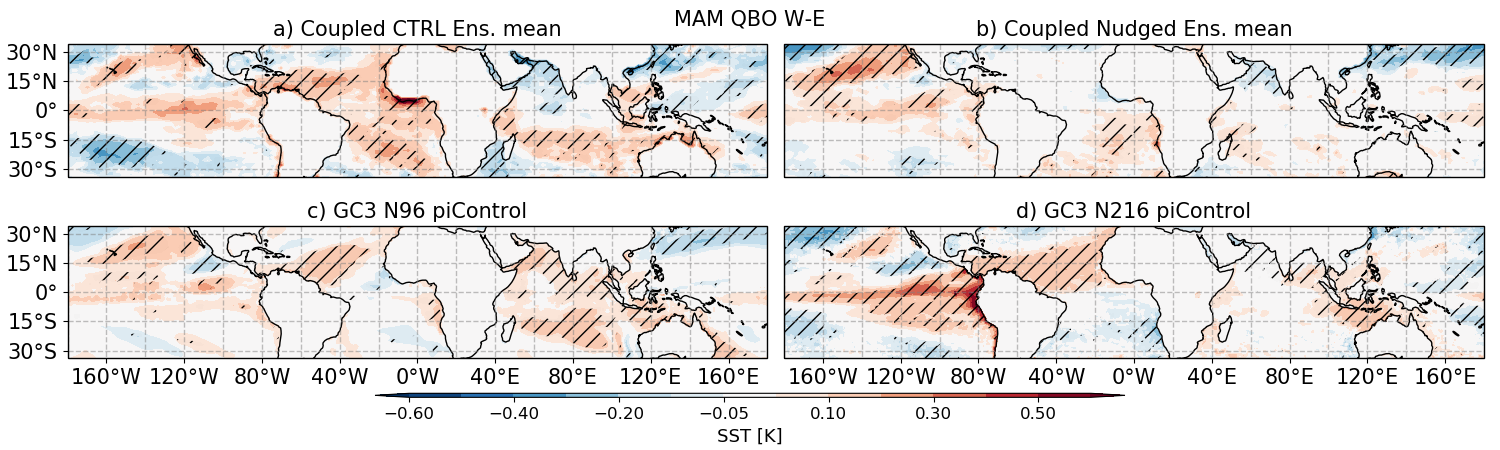
\includegraphics[width=\linewidth]{figures/sstseasonal_mamqbowqboe.png}
\caption[SST response in MAM to the QBO in coupled nudged experiments]{ SST differences between QBO phases in MAM in (a) Coupled Control ensemble mean (2-member), (b) Nudged Coupled ensemble mean (6 members) and in the CMIP6 (c) GC3 N96-pi and (d) GC3 N216-pi.}
\label{fig:sst_mam_coupled}
\end{figure}

The ensemble-mean response shows that averaging over all ensembles results in a weak mean response, with only some differences being statistically significant and different than zero, for example the positive differences found over the coast of Australia and the subtropical Central Pacific. 
In specific seasons, such as MAM (\ref{fig:sst_mam_coupled}), the SST response also appears to be stronger in the tropics in the free-running Coupled Control experiments than in the nudged experiments. 
In MAM, a positive difference found in the Atlantic, Indian and Pacific Oceans in the CMIP6 experiments is also found in the control experiments but this response is weaker in the ensemble-mean of the nudged experiments.
The nudged experiments show a relatively large difference in the eastern subtropical Pacific reaching the coast of California, in agreement with the control experiments.

\begin{figure}[t!]
\centering
 %\noindent
 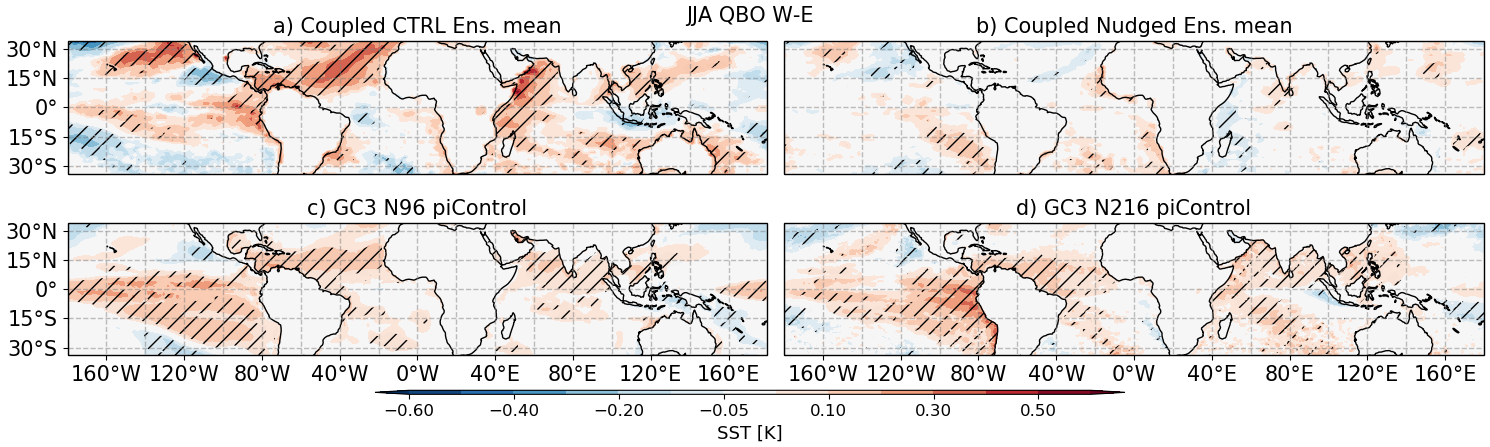
\includegraphics[width=\linewidth]{figures/sstseasonal_jjaqbowqboe.png}
\caption[SST response in JJA to the QBO in coupled nudged experiments]{As in Fig. \ref{fig:sst_mam_coupled} but for JJA.}
\label{fig:sst_jja_coupled}
\end{figure}

The pattern of positive anomalies in the equatorial Central and Eastern Pacific, as well as in the Atlantic Ocean, appears in the control and CMIP6 experiments in most months. 
In boreal summer (Fig. \ref{fig:sst_jja_coupled}), the patterns are particularly strong in the Coupled Control ensemble mean in the Atlantic and Indian Oceans. However, the Nudged experiments show a very weak mean response in the tropics, with only a warm difference found in the western coast of South America. 
For the other seasons, SON and DJF, similar results are found (not shown) in which the ensemble mean of the control experiments agrees well with the CMIP6 experiments, whereas weaker responses are found in the nudged experiments.

These results suggest that the SST response to the phase of the QBO in the nudged experiments is not significantly larger in the experiments with nudging compared to the control or the CMIP6 experiments, especially in equatorial regions. 
In other words, the simulations with a stronger temperature signal associated with the QBO show the  weakest response to the phase of the QBO.
The lack of robust and large patterns of SST anomalies suggests that the precipitation response may also be weaker in the ensemble mean of experiments with nudging, which is the topic of the next section.

\subsubsection{Precipitation response}

\begin{figure}[t!]
\centering
 %\noindent
 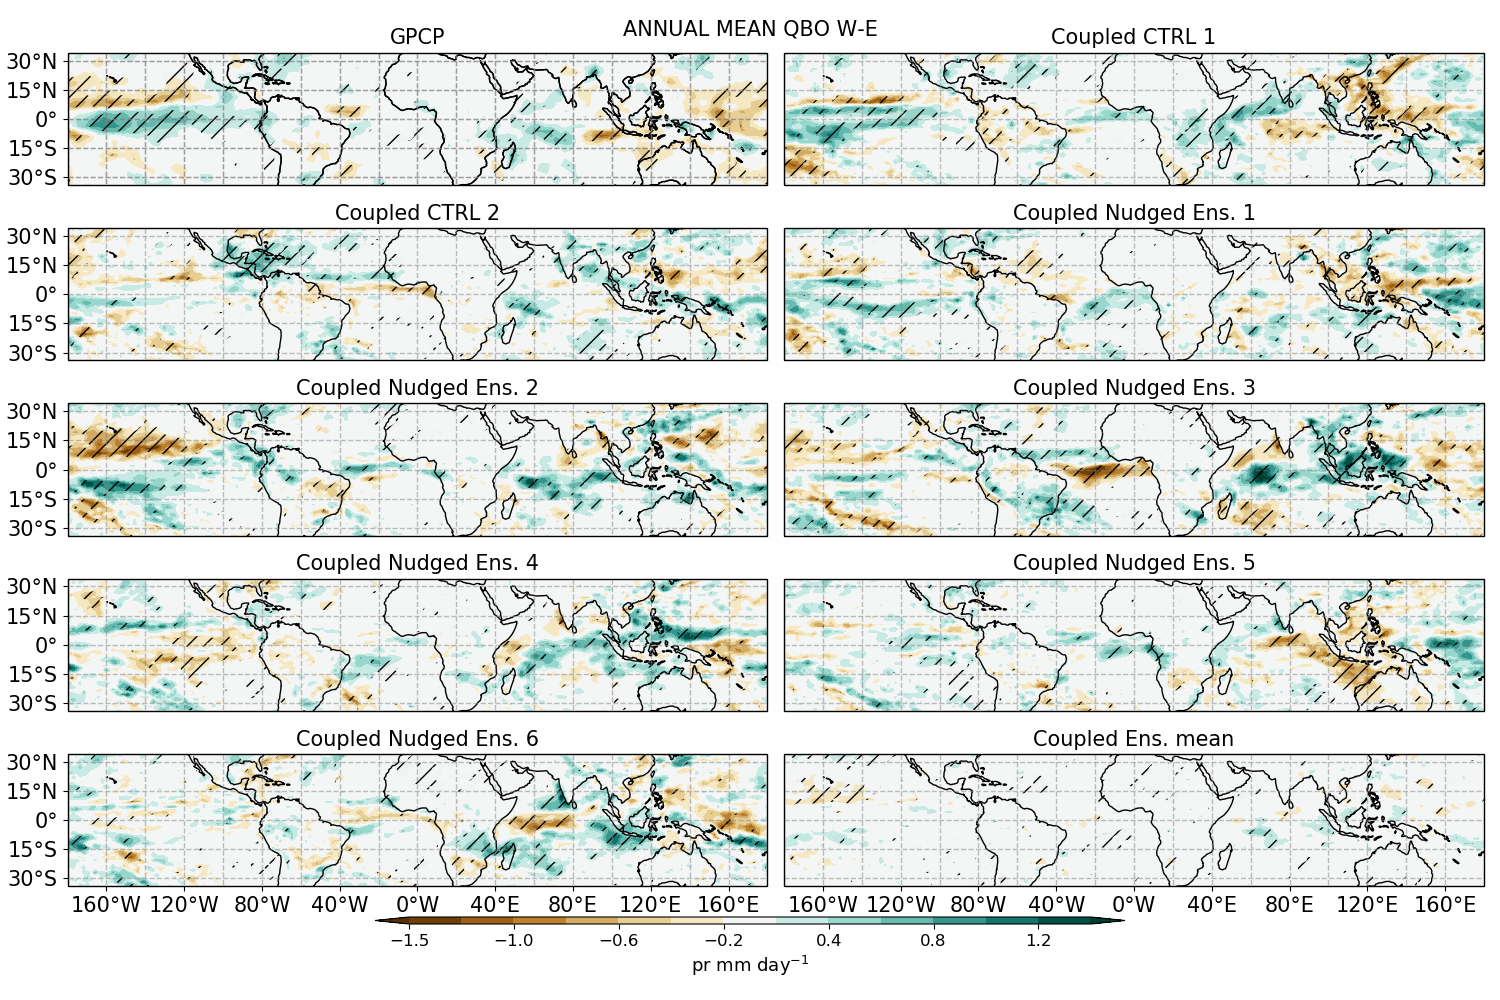
\includegraphics[width=\linewidth]{figures/pr_check_climqbowqboe.png}
\caption[Precipitation response to the QBO in coupled nudged experiments]{ Annual mean precipitation QBO W-E differences in GPCP, Coupled Control, Coupled Nudged ensemble members and the Coupled Nudged ensemble mean. Hatching denotes significance to the 95\% confidence level according to a bootstrapping with replacement test.}
\label{fig:pr_clim_coupled}
\end{figure}


The annual mean difference between QBO phases (Fig. \ref{fig:pr_clim_coupled}) in each coupled experiment reveals a strong variability of the precipitation response, suggesting an important role of long-term variability for these responses. 
In particular, the control experiments show two significant responses: the first control experiment shows a significant El Niño-like response over the Central and Eastern Pacific Ocean, whereas the second control experiment shows a northward shift of the Atlantic ITCZ and a wetter Caribbean Sea.
Precipitation differences in the Indian Ocean and continent are also significant in both of these two coupled experiments, even though the pattern and magnitude of the difference is not a close match, both simulations suggest a wetter western Indian Ocean and continent. 
Note that these three responses found in the Coupled Control experiments in this setup were also observed over the longer GC3 N96 and N216-pi experiments, described previously in Chapter \ref{ch:7-qbo}.

The nudged experiments show different precipitation responses (Fig. \ref{fig:pr_clim_coupled}), with several regions showing significant responses of one sign in one ensemble member and another, also significant, response of an opposite sign in a different ensemble. These varied precipitation responses agree with similarly varied SST differences (Figure \ref{fig:sst_clim_coupled}). In most ensemble members, the stronger responses are seen over the ocean rather than over land.
The nudged ensemble mean shows regions with a significant response but the difference value in signficant regions is too small to be represented by the colorbar, indicating a weak response. 

\begin{figure}[t!]
\centering
 %\noindent
 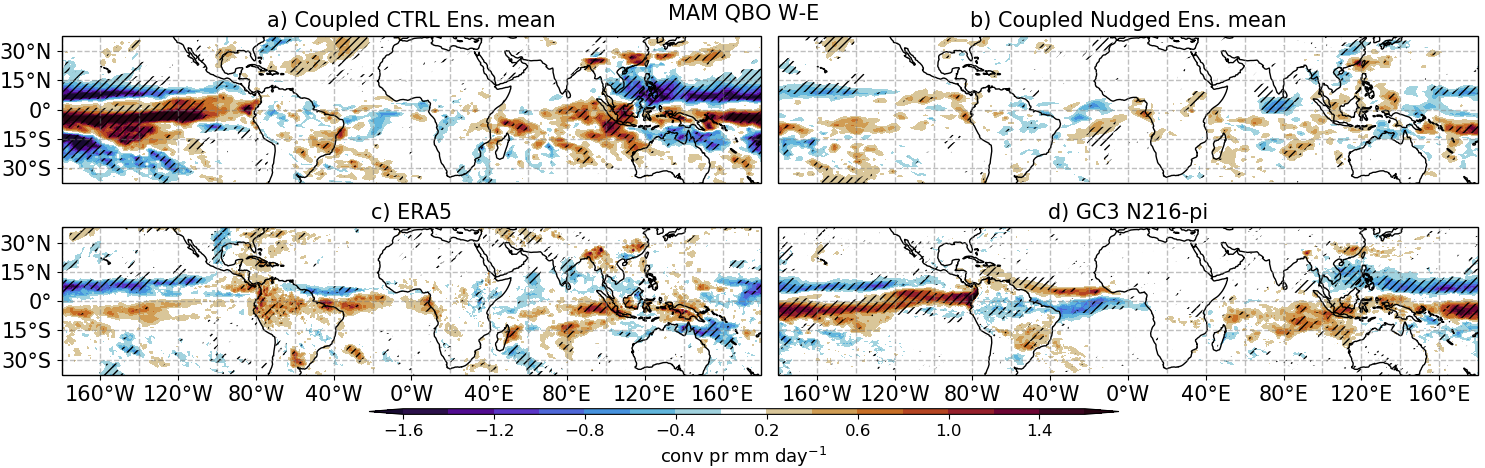
\includegraphics[width=\linewidth]{figures/conv_prseasonal_mamqbowqboe.png}
\caption[ Convective precipitation response in MAM]{As in Fig. \ref{fig:sst_mam_coupled} but for convective precipitation.}
\label{fig:conv_pr_mam_coupled}
\end{figure}

The differences in a specific season are also relatively weak in the ensemble mean of the nudged experiments. 
For instance, in boreal spring, the differences in convective precipitation (Figure \ref{fig:conv_pr_mam_coupled}) show a wetter equatorial Pacific and a drier band at 10$^\circ$N during QBOWthan E in the control ensemble mean and CMIP6 experiments, whereas the nudged experiments only show the dry response. The Coupled Control ensemble mean and CMIP6 experiments agree on the sign and pattern of the response in the Western Pacific and Indian Ocean, characterized by dry anomalies in the Western Pacific ITCZ, the Philippines and the South China Sea, whereas wetter anomalies are observed in the Indian Ocean. 
In contrast, the composite mean results in the nudged experiments show insignificant responses in these above mentioned regions. 



In other seasons, the control experiments also match the results of the CMIP6 experiments, whereas the nudged experiments show a weaker or no response. For example, in boreal summer (Fig. \ref{fig:conv_pr_jja_coupled}) the CMIP6 experiments and Coupled Control experiments show a northward shift of the Atlantic ITCZ, a wetter Caribbean Sea and Indian Oceans and a drier eastern Pacific. The nudged experiments are in reasonable agreement in the Indian Ocean, indicating wetter conditions during QBOWthan E.
Similarly, the effects over the Indian Ocean in SON found for the CMIP6 experiments in section \ref{sq:cmip6_qbo}, are also seen in the Coupled Control experiments, but not in the nudged experiments (not shown).


\begin{figure}[t!]
\centering
 %\noindent
 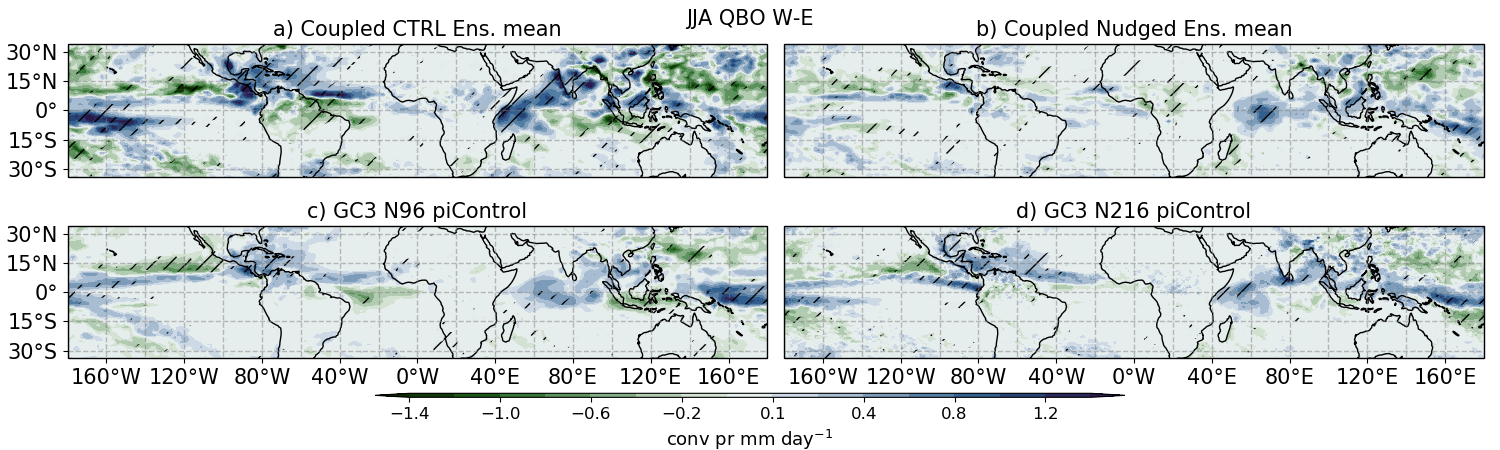
\includegraphics[width=\linewidth]{figures/conv_prseasonal_jjaqbowqboe.png}
\caption[ Convective precipitation response in JJA]{As in Fig. \ref{fig:conv_pr_mam_coupled} but for JJA.}
\label{fig:conv_pr_jja_coupled}
\end{figure}

The results of the precipitation response agree with the previous results that analysed the SST differences. There is no evidence that the nudged experiments result in a stronger surface response to the phase of the QBO, even though the UTLS temperature variability associated with the QBO has been increased and improved in the nudged experiments. 
The next section examines changes to the mean state and variability of the tropical circulation in the nudged experiments, in order to explain the precipitation and SST responses.

\subsubsection{Tropical circulation response and the IOD}

\begin{figure}[t!]
\centering
 %\noindent
 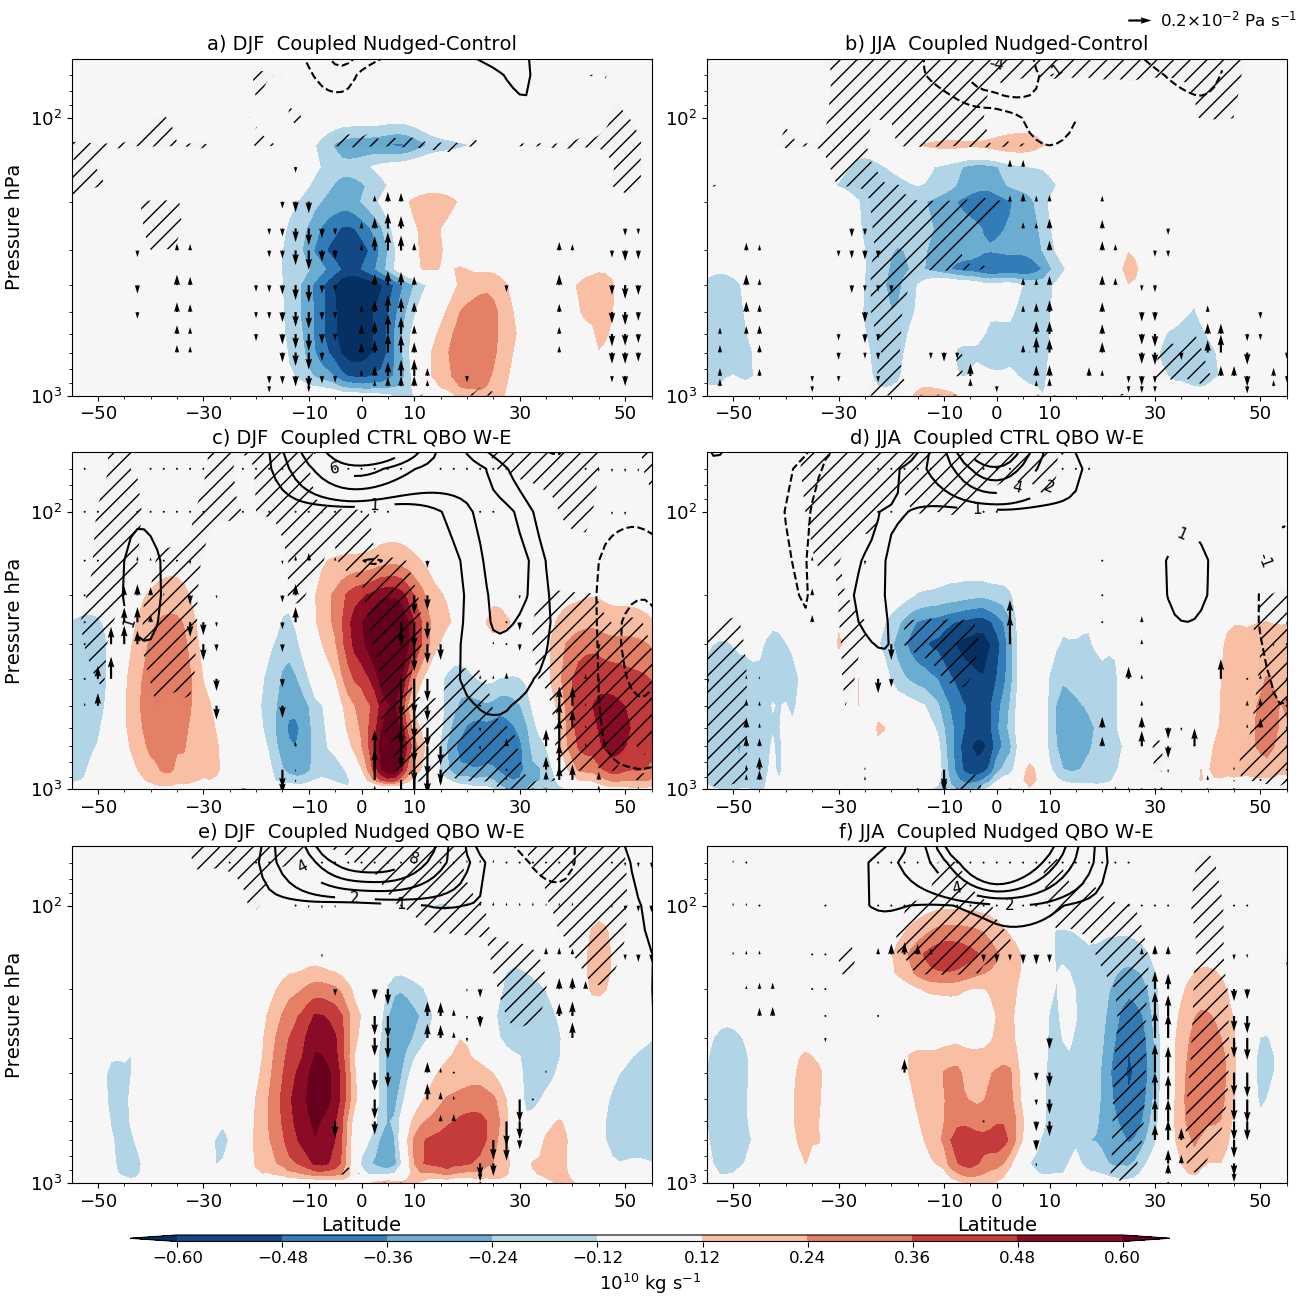
\includegraphics[width=\linewidth]{figures/suite_coupledhadley.png}
\caption[Hadley circulation in coupled nudged experiments.]{Hadley circulation differences in meridional mass streamfunction (shading), zonal wind (contours) and vertical velocity (vectors). (a, b) show the seasonal mean differences between Nudged and Control coupled experiments in (a) DJF and (b) JJA. (c-f) show the QBO W-E differences for the (c-d) Control and (e-f) Nudged experiments for (c,e) DJF and (d,f) JJA. In all panels, hatching denotes significant differences in the streamfunction to the 95\% confidence level according to the bootstrapping method, whereas for the zonal wind and omega, only significant differences are shown.}
\label{fig:hadley_coupled}
\end{figure}

The variability of the tropical circulation in the atmosphere-only experiments was found to be dominated by the SST forcing in the previous section. However, the mean state of the upper-level branch of the Walker circulation was slightly different in the AMIP Nudged experiments compared to the Control. 
To understand whether similar changes to the mean state or variability of the tropical circulation are observed in the coupled experiments, Figures \ref{fig:hadley_coupled} and \ref{fig:walker_coupled} show the impact of nudging on the mean state and variability of the Hadley and Walker circulations, respectively.

The nudging appears to modify the mean state of the Hadley circulation in both DJF and JJA seasons (Figure \ref{fig:hadley_coupled}). Significant changes in the tropical UTLS streamfunction are observed in both seasons, and in DJF changes to the vertical velocity in the tropics suggest a strengthening of the Hadley cell when nudging is applied but very small changes are observed in JJA. 


The difference between QBO W-E in the tropospheric state of the Hadley cell in both seasons is considerably different between Nudged and Control experiments (Figs. \ref{fig:hadley_coupled}c-f). 
In DJF, the Nudged ensemble-mean shows anomalous descent over the 10$^\circ$N latitude band and significantly higher values of the streamfunction at the equator extending into the lower troposphere. Similarly, the zonal wind in this season shows a positive anomaly extending as far down as 500 hPa at 20-30$^\circ$N, indicative of changes to the sub-tropical jet position and strength, documented previously \citep[e.g.][]{garfinkel2010}.

\begin{figure}[t!]
\centering
 %\noindent
 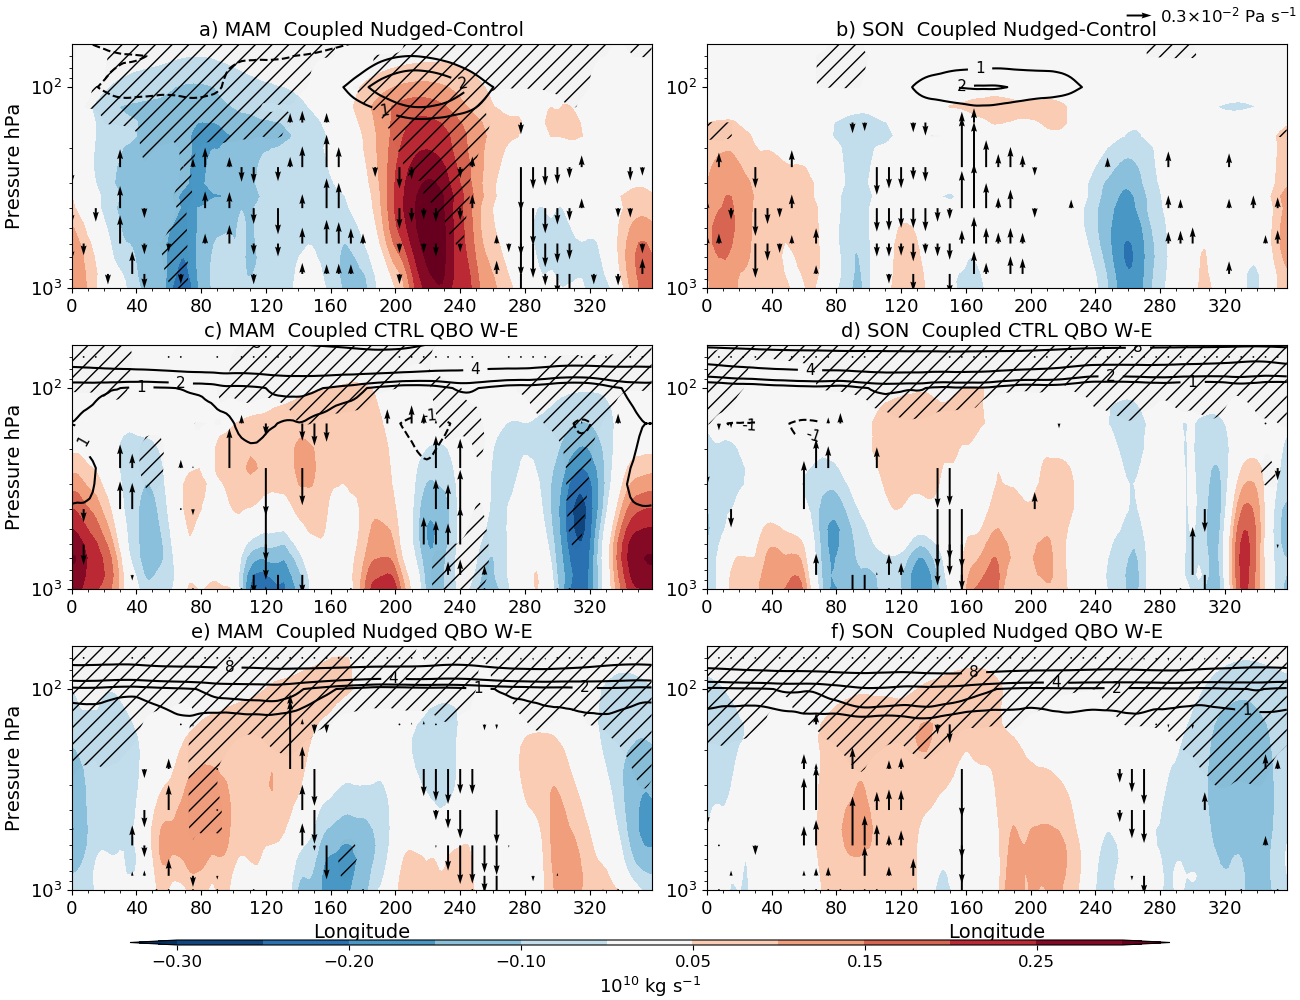
\includegraphics[width=\linewidth]{figures/suite_coupledwalker.png}
\caption[Walker circulation in coupled nudged experiments.]{Walker circulation differences in zonal streamfunction (shading), zonal wind (contours) and vertical velocity (vectors). (a, b) show the seasonal mean differences between Nudged and Control coupled experiments in (a) MAM and (b) SON. (c-f) show the QBO W-E differences for the (c-d) Control and (e-f) Nudged experiments for (c,e) MAM and (d,f) SON. In all panels, hatching denotes significant differences in the streamfunction to the 95\% confidence level according to the bootstrapping method, whereas for the zonal wind and omega, only significant differences are shown.}
\label{fig:walker_coupled}
\end{figure}


The Nudged experiments show stronger zonal wind anomalies in the equatorial stratosphere in both seasons. However, the strengthening of the northern hemisphere subtropical jet during QBO W compared to QBO E, reported in \citep{garfinkel2010} is only found in the Control experiments and not in the nudged experiments. 
Similarly, the differences in the streamfunction and vertical velocity in the nudged experiments appear opposite to that of the Control experiments in DJF. 
The results for JJA are very similar; the nudging results in slightly bigger differences to the control experiments in the stratosphere but weaker responses in the upper-level troposphere in the subtropics.
These results suggest that the process through which the QBO influences the subtropical jets is being affected by the nudging such that the response is weakened or eliminated when the nudging is applied.

%The same contrast is observed in JJA, with the Control and Nudged experiments exhibiting very different responses. Notably, the streamfunction and vertical velocity in the Nudged experiments in this season shows a dipole signal in the Northern Hemisphere with positive and negative anomalies indicating anomalous ascent at 30$^\circ$N and descent at 50$^\circ$N.

The mean Walker circulation is also affected by the nudging (Fig. \ref{fig:walker_coupled}a-b). As in the AMIP experiments, the upper-level zonal wind and streamfunction is modified by the nudging, but in the coupled experiments significant differences are also observed in the lower troposphere over the Indian Ocean and the Eastern Pacific. 
In the UTLS region above the Indian and Pacific Oceans, the nudging is forcing the zonal wind towards ERA5, thus reducing the biases in the model (see e.g. Figure \ref{fig:swalker}). In other words, not only biases in the variability of the zonal winds in the lower stratosphere are alleviated by the nudging but also the mean state of the upper-level branch of the Walker circulation. However, the latter may also mean that the variability of the Walker circulation is overconstrained when nudging is applied. 

The response of the Walker circulation to the QBO is different in the nudged versus control experiments (Fig. \ref{fig:walker_coupled}c-f). In MAM, the QBO W-E differences in the control results suggest a weaker state of the Walker circulation or an El Niño-like pattern with anomalous ascent in the Eastern Pacific under QBO W compared to QBO E whereas the nudged simulations show the opposite. 
In turn, in SON, while the control experiments show anomalous ascent in the western Indian Ocean, the nudged experiments show ascent over the eastern Indian Ocean. 

The nudging appears to modify the mean state and variability of the tropical circulation to a certain extent. However, the differences shown in Figures \ref{fig:hadley_coupled} and \ref{fig:walker_coupled} are relatively small compared to the climatological values,  but clearly some of these differences are still significant. 

Results in Chapter \ref{ch:7-qbo} demonstrated that in the CMIP6 pre-industrial control experiments a statistically significant relationship is found between the IOD and ENSO, and the QBO (Fig. \ref{fig:iod_barplot}). 
Positive events of the IOD and ENSO are more commonly found during QBOW than E, and a convective precipitation index of the IOD and the SST EN3.4 index are also positive during QBOW and negative during QBOE. 
Figure \ref{fig:iod_suites} revisits these relationships in the coupled experiments. 

\begin{figure}[t!]
\centering
 %\noindent
 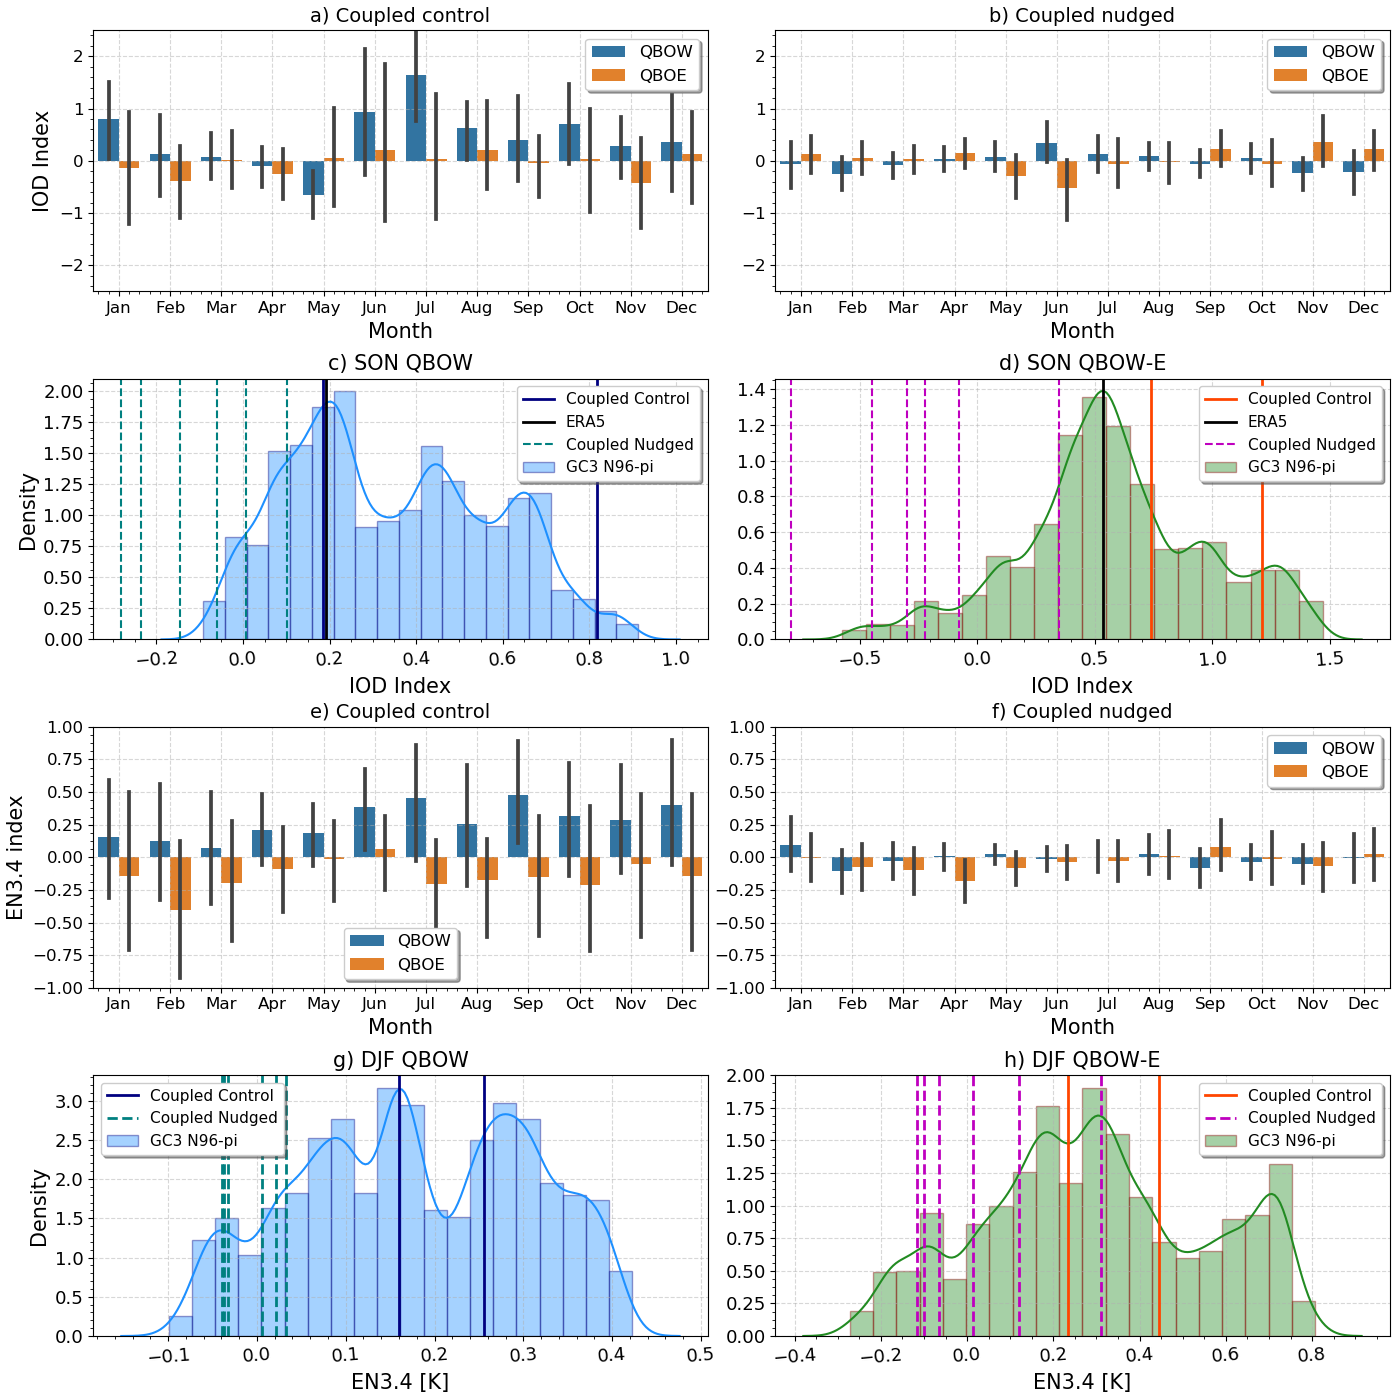
\includegraphics[width=\linewidth]{figures/iod_suites.png}
\caption[IOD and ENSO indices in nudged versus control experiments]{(a, b) Monthly-mean convective precipitation IOD index [mm day$^{-1}$] in coupled (a) control and (b) nudged ensemble-means separated by QBO phase. (c, d) Probability density functions (PDFs) of the IOD convective precipitation index for (c) the mean SON during QBOW months and (d) the SON difference between QBO W-E. The PDF is obtained from the 500 yrs of the GC3 N96-pi by bootstrapping 10,000 times into 35-yr periods and obtaining the averages and differences in each subsample. The mean indices for the Coupled Control and Nudged experiments, as well as for ERA5 are also shown. (e, f) Monthly-mean EN3.4 index [K] in the ensemble mean (e) Coupled control and (f) Coupled Nudged simulations separated by QBO phase.   }
\label{fig:iod_suites}
\end{figure}

The mean IOD index is positive during QBOW and negative during QBOE in the Coupled Control ensemble in boreal fall and early winter (Fig. \ref{fig:iod_suites}a), in agreement with results from the CMIP6 experiments. In contrast, the mean IOD index is close to zero in the Coupled Nudged ensemble without any clear relationship between the index and the QBO phase in any month (Fig. \ref{fig:iod_suites}b). 
These results suggest that no consistent relationship is found across the six ensemble members when nudging was applied in the simulation. 
However, these results may simple be due to sampling of the ocean-atmosphere state used for the nudged experiments, in other words, possibly due to decadal variability in the GC3.1 configuration.

For that reason, the CMIP6 GC3 N96-pi is used to investigate whether the results of the Nudged and Control experiments are also seen in periods of similar length in that long 500 yr simulation. While this comparison is not perfect due to differences in ocean resolution and forcing, the model setup and parametrisations, and atmospheric resolution is otherwise the same between GC3 N96-pi and these experiments. 
The simulation is repeatedly sampled at random for 35 yr continous periods, and the SON IOD index is computed each time to construct a probability distribution.  

Figure \ref{fig:iod_suites}c shows that the IOD index during QBOW in GC3 N96-pi is more frequently positive, as shown in the previous section, but in some 35-yr periods a negative mean index during QBOW can be observed in this simulation. The two Coupled Control simulations and ERA5 show a positive mean IOD index during QBOW whereas four out of the six Coupled Nudged simulations show a negative index. 

Chapter \ref{ch:7-qbo} showed that in ERA5 and the three pre-industrial control experiments of the MOHC, positive IOD indices and events are more frequent during QBO W, and the opposite is true for QBOE. Figure \ref{fig:iod_suites}d  shows that the difference in the IOD index during SON between the two QBO phases is most frequently positive in GC3 N96-pi.  
Results from ERA5 and the two Coupled Control simulations also show a positive difference of 0.6 mm day$^{-1}$ for the reanalysis and up to 1.3 mm day$^{-1}$ for one of the control simulations. 
In contrast, the nudged experiments are found to the left of the mean of the PDF of GC3 N96-pi.
These results indicate that the QBO W-E response in the IOD in the nudged experiments is  weaker response and of a different sign compared to the results in ERA5, the pre-industrial control experiments of CMIP6, and the two Coupled Control experiments used in this chapter. 

Finally, the ENSO index is found to be positive in the Control experiments, as in the MOHC CMIP6 experiments and in ERA5, but no robust relationship is found in the Nudged experiments. As with the CMIP6 experiments, the Coupled Control EN3.4 index is positive during QBOW and negative during QBOE throughout most of the year. However, there seems to be no relation between the QBO and the EN3.4 index in the nudged experiments. 
Overall, these results suggest that the relationships between the QBO and the IOD and ENSO observed in the CMIP6 or Control experiments are not found in the Nudged experiments, which show little-to-no relationship between these two indices and the QBO phase.

\section{Summary and discussion}

Tropical teleconnections associated with the QBO are difficult to understand in observations due to the relatively large observational uncertainty and the influence of ENSO. 
In models, biases in the QBO also complicate the investigation of tropical circulation and the surface response to the QBO, largely because the key aspects of the QBO that are hypothesized to the influential for stratospheric-tropospheric coupling in the tropics are poorly represented by most models. 
This chapter investigates the influence of the QBO over tropical climate through nudging experiments using the MOHC UM which aim to improve the representation of the QBO in the lower stratosphere while also removing any possible influence of the troposphere on the QBO.  

The nudging technique results in simulations that exhibit a more realistic representation of the variability of the QBO winds and temperature in the lower stratosphere. In other words, the nudging experiments simulate a stronger response of the UTLS temperature to the QBO. 
However, in the atmosphere-only setup, the nudging does not modify the variability of precipitation and OLR as the SST variability imposed dominates. 
Sensitivity tests with the imposed SSTs shifted by one year demonstrated that the QBO response requires the presence of the correct SSTs.

In the coupled experiments, the control simulations largely agree with the results found in the first part of the chapter using the CMIP6 versions of the model (as expected). However, in the nudged experiments, the tropical SSTs and precipitation show no consistent difference between the QBO phases across the ensemble-mean.  Further evidence that analyses the circulation response and on the IOD and ENSO indices confirms that there is no indication that the nudging has made the response to the QBO stronger, or indeed closer to the observed response. In fact, the imposed nudging appears to have disrupted the mechanism that causes the QBO influence at the surface in equatorial latitudes. 

One explanation for the nudged results may be that the static stability mechanism, the most cited mechanism in the literature \citep{collimore2003,liess2012,nie2015,gray2018,lee2018}, may not be the dominant factor that relates the QBO to the tropical surface. 
Specifically, in ERA5, the temperature signal becomes very small at levels lower than 125 hPa, and the 1 K difference at 100 hPa may not be large enough to modify the static stability of the whole convective profile in a significant manner.

An alternative hypothesis is that by nudging we have modified the mean state of the Walker circulation, as was demonstrated in this chapter. Therefore, the teleconnections operating through the Walker circulation simulated by the model become different in the nudged experiments, either because of the relatively minor mean-state change or because Walker circulation-QBO feedbacks have been disrupted by the relaxation. Note that the nudging was only applied to the zonal winds above 90 hPa, so while the zonal winds of the QBO and upper arm of the Walker circulation may be consistent, the meridional and vertical winds in the troposphere are unconstrained.  

Another explanation could be that the relationships found in the free-running versions of the model are not due to a causal influence from the QBO downward (top-down) but rather a result of the influence of tropical convection on the phase of the QBO. Studies \citep[e.g.][]{schirber2015,christiansen2016} have shown that the tropical wave activity, largely modulated by ENSO, can influence the descent rate and season of phase change of the QBO. Perhaps then, the ENSO-QBO relationship found in the CMIP6 models is lost in the nudged experiments because the forcing of ENSO cannot influence the QBO. 

Future work could improve from this chapter in several ways. 
Firstly, instead of using a nudging scheme, which is not ideal since it does not target and improve the physical mechanisms,  an improvement of the representation of tropical waves associated with deep convection would be better and simultaneously improve the representation of the QBO characteristics as well the teleconnections. One such example is seen in \cite{serva2021} which compares simulations with different gravity wave schemes resulting in different properties of the QBO but also precipitation responses in the tropics.
 
Secondly, the nudging was applied in a relatively coarse resolution configuration (N96) but the results may be different in a medium-resolution (N216) configuration due to the improvement in the tropospheric dynamics that was found in Chapter \ref{ch:4-ams}\. 
Additionally, the relaxation in this chapter was done at all grid-points, due to model constraints, however, other types of nudging have been applied, for example by \cite{martin2021}, so that only the zonal mean (zonal wavenumber of zero) is nudged, allowing the wave disturbances (higher wavenumbers) to freely evolve. In this way, the wave disturbances in the lower stratosphere would be more consistent with the wave disturbances generated in the troposphere. Nudging in a zonal-mean sense using a model that can internally generate a reasonable QBO could provide more answers to some of the results in this chapter.

